% TEMPLATE for Usenix papers, specifically to meet requirements of
%  USENIX '05
% originally a template for producing IEEE-format articles using LaTeX.
%   written by Matthew Ward, CS Department, Worcester Polytechnic Institute.
% adapted by David Beazley for his excellent SWIG paper in Proceedings,
%   Tcl 96
% turned into a smartass generic template by De Clarke, with thanks to
%   both the above pioneers
% use at your own risk.  Complaints to /dev/null.
% make it two column with no page numbering, default is 10 point

% Munged by Fred Douglis <douglis@research.att.com> 10/97 to separate
% the .sty file from the LaTeX source template, so that people can
% more easily include the .sty file into an existing document.  Also
% changed to more closely follow the style guidelines as represented
% by the Word sample file. 

% Note that since 2010, USENIX does not require endnotes. If you want
% foot of page notes, don't include the endnotes package in the 
% usepackage command, below.

% This version uses the latex2e styles, not the very ancient 2.09 stuff.

\documentclass[letterpaper,twocolumn,10pt]{article}
\usepackage{usenix,epsfig,endnotes}
\usepackage{xcolor}
\usepackage{amssymb}
\usepackage{graphicx}
%\newcommand{\nancomment}[2][blue]{\textcolor{#1}{\textit{#2}}}
\newcommand{\nancomment}[1]{\noindent\textcolor{blue}{\bf $\blacksquare$ Nannan: #1}}
\newcommand{\vcomment}[1]{\noindent\textcolor{orange}{\bf $\blacksquare$ Vasily: #1}}
\begin{document}

%don't want date printed
\date{}

%make title bold and 14 pt font (Latex default is non-bold, 16 pt)
\title{\Large \bf Large-Scale Analysis of Docker Registry Dataset }

%for single author (just remove % characters)
\author{
{\rm Your N.\ Here}\\
Your Institution
\and
{\rm Second Name}\\
Second Institution
% copy the following lines to add more authors
% \and
% {\rm Name}\\
%Name Institution
} % end author

\maketitle

% Use the following at camera-ready time to suppress page numbers.
% Comment it out when you first submit the paper for review.
\thispagestyle{empty}

%\subsection*{Abstract}
\begin{abstract}

\vspace{-6pt}
%
The rapidly growing number of container images and the associated storage
performance and capacity requirements are the key obstacles to efficiently
scaling Docker registries.
%
Though the real-world images contain a tremendous amount of duplicate data,
modern registries cannot effectively eliminate the duplicates due to the
compressed format of the images.
%
In this paper, we propose a new Docker registry architecture, \emph{\sysname},
that integrates deduplication into the Docker registry.
%
\sysname supports several configurable deduplication modes that provide
different levels of storage efficiency, durability, and performance, as desired
by different use cases.
%
Further, to mitigate the negative impact of deduplication on the image download
and upload times, \sysname introduces a two-tier cache with a novel
user-access-history-based prefetch algorithm. 
%
Under real workloads, \sysname saves up to XXX\% of storage space while keeping
the latencies within the XXX\% of the original registry.

%The approach enables it to achieve a $96$\% hit ratio and save $56$\% more
%cache space.

%Based on our 

%sustaining and scaling container systems in the face of exponential growth is challenging. 
%%
%For example, Docker Hub~\cite{docker-hub}---a popular public container registry---stores more than~2 million public repositories. These repositories have grown at the rate of about $1$ million annually---requiring provisioning an additional 2.5~TB of storage per week on average---and the rate is expected to increase.
%%
%This puts intense pressure on Docker registry storage infrastructure, but the problem has so far remained largely unexplored.
%

\end{abstract}

%we predict  
%Overall,  
%to model the deduplication for estimating the deduplication effect on performance and storage savings, especially in terms of deduplication rate and deduplication overhead. We propose to use Markov decision process to find optimal solution that can maximize the storage saving and minimizing the cost in terms of performance degradation. Our solution will largely reduce the amount of redundant data in container storage systems and outperform the state-of-art deduplication techniques without any performance overhead.

%and evaluate
%the potential of file-level deduplication in the registry.
%
%Our analysis reveals that 
%
%We then present the design of \sysname---a Docker registry with file deduplication
%support---and conduct a simulation-based analysis of its performance implications.

\section{Introduction}
 
Containers have become a prominent solution for deploying modern applications because to their tight isolation, low overhead, and efficient packaging of the execution environment~\cite{docker}.
Containers are the running instances of \emph{images} which contain the complete runtime environment for an application.
An image comprises a set of shareable and content addressable \emph{layers}.
% and is stored in Docker \emph{registry}. 
Each layer is a set of files that are compressed in a single archive. 
Docker images/layers are stored in an online store called Docker registry~\cite{docker-hub} and accessed by clients as needed.
%As layers are the building blocks of images, they can be shared among multiple images. 
Since layers are uniquely identified by a collision-resistant hash of its content, 
no duplicate layers are stored in the registry.
Many container registries use remote cloud storage like S3~\cite{s3}, 
Microsoft Azure~\cite{azure}, and OpenStack Swift~\cite{swift} as their backend storage systems~(Figure~\ref{fig:without-dedup}).
%For example, Google container Registry~\cite{GoogleContainerRegistry} stores images on Google cloud storage while
%IBM container registry uses IBM cloud to manage image storage.

The amount of images stored in Docker registries is increasing dramatically.
%Docker registries store a large amount of images and with the increasing popularity of Docker, registries continue to grow. 
For example, Docker Hub~\cite{docker-hub}---a popular public registry---stores more than~2 million public repositories that host one or more images. 
We observed that the number of public repositories grows by around~1 million annually. 
We estimate that~1 million annual growth in the number of repositories 
amounts to about~130\,TB storage space required per year.
%Moreover, 
%just storing~130\,TB worth of Docker images on Google cloud will cost around~\$14,000 per month~\cite{GoogleCloudStoragePricing}.
This massive amount of image dataset presents great challenges for Docker registry storage infrastructure and so far has remained largely unexplored.
%Then, the 1 million annual growth in the number of repositories amounts to about 130\,TB, costing around~\$15,000 a month.

\paragraph{Deduplication}
Our analysis of around~47\,TB (167\,TB uncompressed) of Docker images downloaded from Docker Hub,
which in total contain over~5 billion files, reveals that
that only~3\% of the files are unique while others are redundant copies. 
%Since many Docker images share many underlying layers, 
This suggests that current layer sharing mechanism cannot efficiently remove data duplicates.
%current
% considerable file-level redundancy across different images is not mitigated by Docker's existing layer sharing mechanism.
Many cloud storage systems already implemented deduplication to effectively eliminate redundant data.
%\NZ{let use redundant data instead of redundancy}
For example,
Google cloud and AWS, 
perform in-line data deduplication transparently.\NZ{use a new example}
However, existing deduplication techniques cannot be directly applied to the image storage system 
because of unique dataset in the Docker registry: compressed layers. 
In contrast to uncompressed files, compressed files have a lower deduplication ratio. 
So layers should be decompressed before performing deduplication.

As shown in Figure~\ref{fig:with-dedup}, 
after decompression and simple file-level deduplication, the unique files may get scattered on
multiple servers. 
To restore a layer,
the layer's containing files should be first fetched from multiple servers, then compressed as a layer
and sent back to the client.
The extra network, I/O, and computation latency will slow down the response time for pulling an image.

%Without deduplication (Figure~\ref{fig:without-dedup}),
%the average latency for requesting a layer is around~2\,s for layers with size less than~50\,MB.
%The latency increases to~12\,s when deduplication is implemented in the backend storage system.
%Furthermore, Docker registry performance drops down dramatically for bigger layers.

%We observe that the average latency for requesting layers larger than~50\,MB and smaller than~1\,GB
%is around~128\,s. The latency worsens when dedupliation is implemented, with an average around~800\,s.
%incurs a considerable additional overhead on layer pull time and thus affecting the overall container startup time. 
%A solution would be to decompress the layers before applying deduplication on Docker registries.
 
%Therefore, in this paper, we propose a new Docker registry architecture,~\sysname,
%that integrates caching and deduplication with Docker registries to address the aforementioned obstacles.
%low restore latency %adaptive%
% deduplication framework for Docker registries. 

\paragraph{Caching}
Large container registry service providers like Google and IBM use regional private registries across the world to facilitate a fast and high-availability service~\cite{GoogleContainerRegistry,ibmregistry}.  
This geographical distribution allows users to store images near their compute instances and experience a fast response time. 
Deploying these registries as a cache, temporarily storing popular layers,
to improve pull latency may be intuitive.
%Although cache has been studied as web cache or proxy cache, 
However, there are unique challenges in integrating a cache with deduplication in Docker registry.
%%%%
%we can use registry as a web/proxy cache because registry already has been deployed regionally close to clients to speedup performance. although there are so many works on web/proxy cache but you cannot just use it with docker registry because of the following challenges. 
%%%%
First, we observe that layer sizes vary from a few MB to several GB and that majority of layers are around several MB.
A small main memory cache cannot accommodate many popular layers.
Second, 
Although layer pull requests are heavily skewed, we observed that the duration between two subsequent requests is too long. 
Meaning, if we cache a layer, we might need to wait hours to get a hit on that layer.

\paragraph{~\sysname}
In this paper, we propose a new Docker registry architecture,~\sysname,
that integrates caching and deduplication with Docker registries to address the aforementioned obstacles.
%To address these issues,
~\sysname~embodies a two-tier heterogeneous cache architecture 
comprising a layer buffer and a file cache to hold even more popular layers:
The layer buffer stores popular layers in main memory while the file cache stores 
the \emph{deduped} unique files for the victim layers that are evicted from the layer buffer on a 
flash-based storage system to improve cache space utilization.
Moreover, we proposed a user-based cache algorithm to improve the cache hit ratio 
because we observed that user active time is more predictable.

%Moreover, to improve layer pull performance, we design a user behavior based cache. 
%The cache adaptively stores a certain amount of active users' layers, in a layer buffer, to speed up active users' pull time. 
%The cache also selectively stores a few popular \textit{shared} and \textit{deduplicated} files, in a file cache, to accelerate the layer restoring process. 
%The rationale behind the user behavior based cache is that, instead of only focusing on layer-level access pattern, 
%we consider the user behavior for cache replacement because users' behavior is more predictable than layer access pattern. 
%Moreover, users are the ones who issue the layer/manifest pulls and pushes.  
%For this reason, our cache replacement policy is an adaptive heuristic, top-down decision making process driven by users' behavior.
%During cache eviction, we evict the least recently accessed layer from a set of candidate layers exclusively referenced by the least recently active users to make room for new users' layers. 
%After an inactive user's layer is evicted from the layer buffer, based on our algorithm, it can either be discarded or hosted in the file cache. For the latter, the layer will undergo offline decompression and file-level deduplication.
%For the incoming new users, we prefetch a number of their repositories along with their containing layers based on their access probabilities.

We evaluate our proposed design, \sysname. 
\sysname~acheives a hit ratio~20\% higher than that of traditional LRU. 
%by conducting a preliminary simulation-based study. Our study aims to explore the feasibility/benefits of deduplication and quantify the overhead it introduces.
\HA{plz add preliminary results}.  

\begin{figure}[t]
	\centering
		\begin{minipage}{0.225\textwidth}
			\centering
			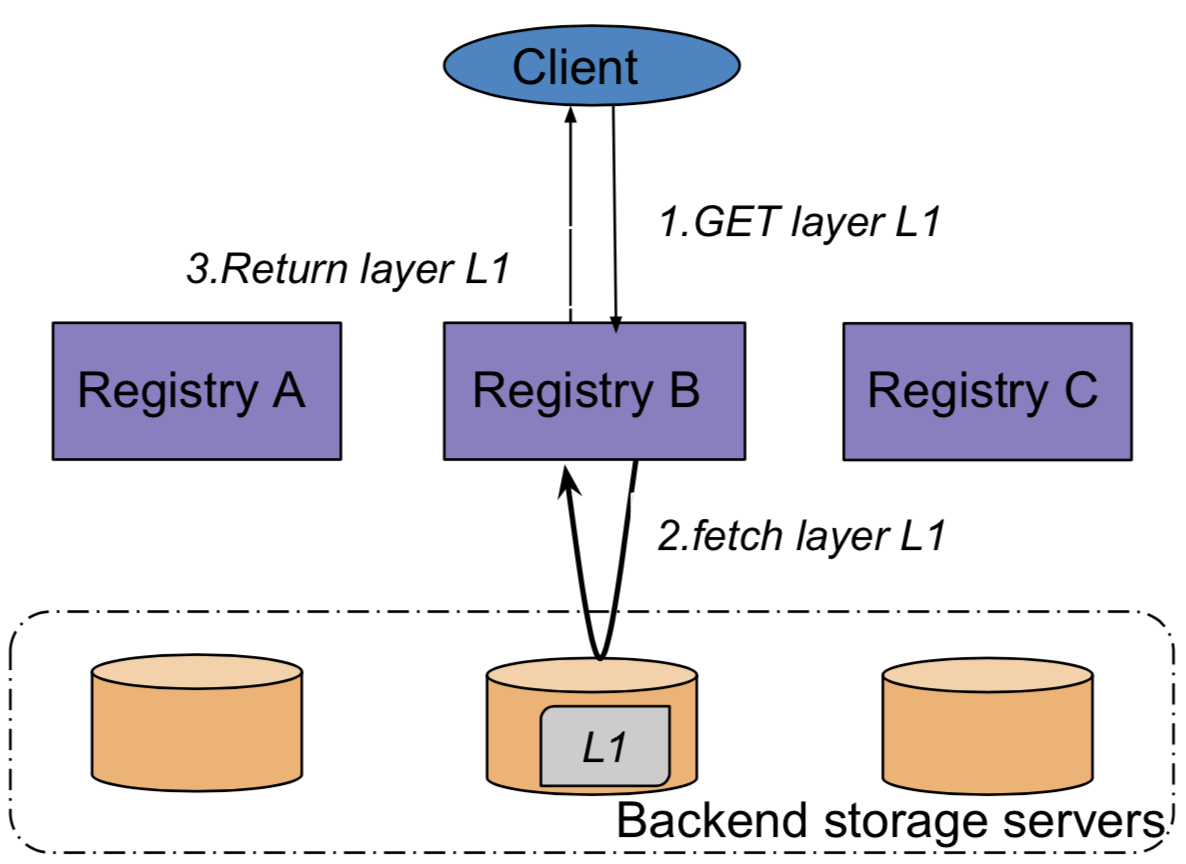
\includegraphics[width=1\textwidth]{graphs/nodedup.png}
			\caption{CDF of layer reference count.}
			\label{fig:ref_count}
		\end{minipage}
	\begin{minipage}{0.225\textwidth}
		\centering
		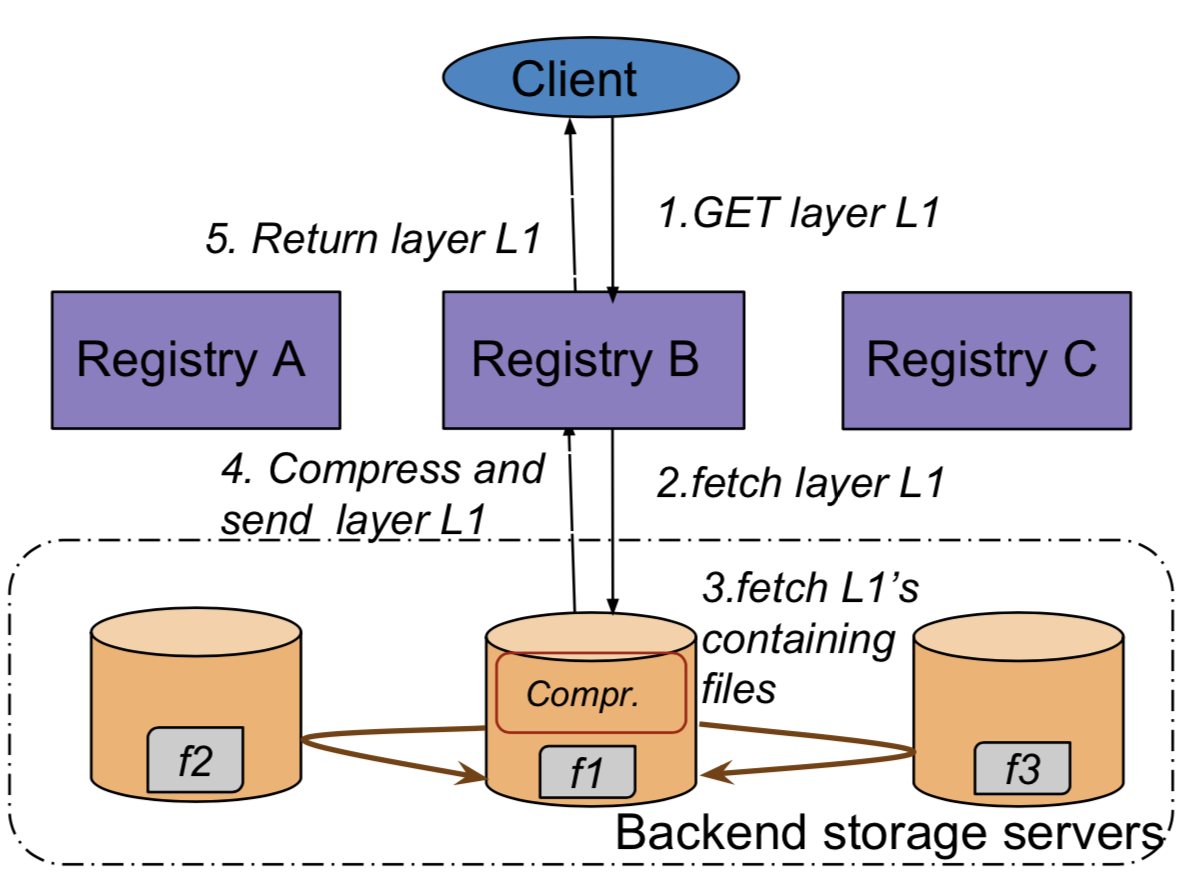
\includegraphics[width=1\textwidth]{graphs/dedup.png}
		\caption{CDF of compress. and uncompress. layer size.}
		\vspace{-3pt}
		\label{fig:nodedup-vs-dedup}
	\end{minipage}
\end{figure}

%\HA{need to mention Figure~\ref{fig:without-dedup} and Figure~\ref{fig:with-dedup}}

The organization of this paper as follows: 
We explain relevant Docker details along with observations and current deduplication practices in production registries in~\cref{sec:background}.
We present~\sysname~in~\cref{sec:\sysname} and ~\sysname's preliminary evaluation in~\cref{sec:Evaluation}. 
We discuss related work in~\cref{sec:related}.
Lastly, we conclude and discuss in~\cref{sec:conclusion} and~\cref{sec:discussion}.

%%%%%%%%%%%%%%%%%%%%%%%%%%%%%%%%%%%%%%%%%%%%%%%%%%%%%%%%%%%%%%%%%%%%%%%%%%%%%%
%                                                                            %
%                                OLD INTRO                                   %
%                                                                            %
%%%%%%%%%%%%%%%%%%%%%%%%%%%%%%%%%%%%%%%%%%%%%%%%%%%%%%%%%%%%%%%%%%%%%%%%%%%%%%

%\emph{Containers}~\cite{process-containers-linux} have recently gained
%significant traction due to their low overhead, fast deployment, and
%the rise of container management frameworks such as Docker~\cite{docker}.
%%
%Polls suggest that 87\% of enterprises are at various stages of adopting
%containers, and they are expected to constitute a \$2.7 billion
%market by 2020~\cite{container-grow-by2020}.
%
%Docker combines process containerization with efficient and effective packaging
%of complete runtime environments in so called {\em images}.
%%
%Images are composed of shareable and content addressable {\em layers}.
%%
%A layer is a set of files, which are compressed in a single archive.
%%
%Both images and layers are stored in a Docker \emph{registry} and accessed by
%clients as needed.
%%
%Since layers are uniquely identified by a collision-resistant hash of
%their content, no duplicate layers are stored in the registry.
%
%Registries are growing rapidly.
%%
%For example, Docker Hub~\cite{docker-hub}, the most widely used registry,
%stores more than 500,000 public image repositories comprising over 2 million
%layers and it keeps growing.
%%
%Over a period from June to September 2017, we observed a linear growth of the number
%of images in Docker Hub with an average creation rate of 1,241 repositories per day.
%%
%We expect this trend to continue as containers gain more popularity.
%%
%This massive image dataset presents challenges to the registry storage
%infrastructure and so far has remained largely unexplored.
%
%In this paper, we perform the first large-scale redundancy
%analysis of the images and layers stored in Docker Hub.
%%
%We downloaded 47\,TB (167\,TB uncompressed) worth of Docker Hub images,
%%
%which in total contain over 5 billion files.
%%
%Surprisingly, we found that only around 3\% of the files are unique
%while others are redundant copies. This suggests that current layer
%sharing cannot efficiently remove data duplicates.
%%
%We further analyzed the reasons for the high number of redundant files
%and found, for example, that different Docker images often
%contain the same source code from external public repositories
%(e.g., GitHub~\cite{github}).
%%
%%As there are no official images containing this source code, users manually add
%%it to their images, resulting in different layers which cannot be reused.
%
%Given our findings, we propose \sysname, a file-level content addressable storage
%model for the Docker registry.
%%
%\sysname\ unpacks layer tarballs into individual files and deduplicates them.
%%
%When a Docker client requests a layer, \sysname\ dynamically reconstructs the
%layer from its constituent files.
%%
%To assess the feasibility of our design, we conduct a simulation-based
%evaluation of \sysname. 
%%
%The simulation results show that \sysname\ improves the deduplication
%ratio from 1.8$\times$, provided by layer sharing, to 6.9$\times$.
%%provided by file-level deduplication.
%%
%While \sysname\ comes with some overhead 
%%when retrieving layers from the registry
%caused by the need to decompress and reconstruct layers, we found,
%for example, that for
%layers less than 10\,MB (around 60\% of all layers) the overhead of
%retrieving a layer is less than 1\,s.
%%
%For larger layers, we propose several optimizations to reduce overhead.
%\VT{Here we need to add 1-2 *most interesting* performance-related findings.}

%
%The simulation result show that 
%(1)~processing layers in
%parallel can largely improve throughput. For example, 80\% of file-level deduplication time is
%less than 9.09 s per layer and by processing 60 layers in parallel, our one-node
%prototype can process about 3 layers per second.
%
%\LR{That sounds like we actually ran the deduplication and not just simulated it?
%Did we perform more of an \emph{emulation}?}
%
%(2) Fast compression methods can mitigate pull overhead caused by re-compression
%because files are required to be re-compressed as a compressed layer archival file to serve
%the incoming pull requests.
%

%
%We make three major observations:
%
%\begin{compactitemize}
%
%\item Only 10\% of layers are referred to by more than one image, 
%meaning that layer-level content addressability is not enough to
%effectively reduce storage utilization in the registry.
%\DIM{Should we also provide the capacity \%?}
%
%\item A large amount of files are shared across layers and images,
%resulting in only 3\% of unique files.
%\DIM{Should we also provide the capacity \%?}
%
%\item Source code and scripts have a high deduplication ratio
%(\textbf{$31.25\times$} for source codes and \textbf{$50\times$} for scripts),
%which can result in executable and object file duplicates.
%
%\end{compactitemize}


%%%%%%%%%%%%%%%%%%%%%%%%%%%%%%%%%%%%%%%%%%%%%%%%%%%%%%%%%%%%%%%%%%%%%%%%%%%%%%
%                                                                            %
%                                OLD INTRO                                   %
%                                                                            %
%%%%%%%%%%%%%%%%%%%%%%%%%%%%%%%%%%%%%%%%%%%%%%%%%%%%%%%%%%%%%%%%%%%%%%%%%%%%%%

%Finally, we proposed and implemented Docker registry design that performs
%deduplication.
%%
%In our thorough redundant analysis and characterization of the xxxx images,
%with xxxx layers and xxxx files, we investigated the following four research
%questions (RQs):
%
%\begin{compactitemize}
%%
%\item How much redundant data stored in layers, images, and registry? Although
%layer-level address content addressable storage is adopted by Docker, we do not
%know whether  this coarse-grain layer-level content addressable storage (LLCAS)
%can efficiently reduce duplicates, and how much redundant data is stored in
%layer, image, and registry.
%%
%\item What are the redundant files and why there are so many redundant files?
%We aim to identify what are the redundant files that users mostly replicate.
%%
%Such information will provide Docker designer knowledge (user behavior) to
%better develop and optimize Docker container and Docker registry storage
%system.
%%
%\item What are the challenges faced by Docker registry and engine designer? By
%characterizing and analysis all the image metadata, we aim to identify the
%challenges' faced by registry designer and guide designers'optimization and
%users' development.
%%
%\item How to reduce the redundant files? We aim to propose a file-level content
%addressable model to reduce the redundant files by using file-level dedup while
%maintaining a good performance.
%%
%\end{compactitemize}
%
%The significance of this work are (1) our empirical evidence that large amount
%of redundant files exist in layers, images, and registry and layer-level
%content addressable storage is not efficient to remove redundant files;(2)
%findings about what are the redundant files and why there are so many redundant
%files exist;(3) first in-depth characterization on image dataset (union file
%systems)(4) a file-level content addressable model that can efficiently remove
%redundant copies while maintain a good performance.

%For years, virtual machines served as a cornerstone of computing resource
%virtualization both on premises and in the cloud~\cite{rosenblum2005virtual}.
%%
%Recently, however, \emph{container-based} virtualization started to gain
%significant traction~\cite{process-containers-linux}.
%%
%According to polls, over 87\% of enterprises are at various stages of adopting
%containers; analysts also predict that by 2020, containers will constitute a
%lucrative \$2.5 billion market~\cite{container-grow-by2020}.
%
%
%
%At its core, container is a set of processes which are isolated by the operating
%system kernel in terms of visibility and resources. This allows containers to share
%the same kernel without being aware of each other.
%%
%For example, Linux performs visibility isolation (for user identifiers, file systems,
%network, etc.) using namespaces~\cite{man-namespaces} and enforces resource
%utilization constraints with control groups~\cite{kernel-doc-cgroups}.
%%
%Compared to virtual machines, containers use less memory and storage, are much
%faster to start, and typically cause less execution
%overhead~\cite{felter2015updated, Disco, HypervisorsvsLightweight}.
%
%The rapid increase in use of container technology was largely made possible by
%container management frameworks, with Docker being one of the most popular
%solutions~\cite{docker}.
%%
%Docker combines process containerization with efficient and effective runtime
%environment packaging.
%%
%Software is packaged in container \emph{images}, each consisting of several
%read-only \emph{layers} and a manifest which describes container metadata, \eg
%what layers make up an image and which command to run at container startup.
%%
%Read-only layers can be shared between different images and encapsulate
%file-system trees for dockerized processes.
%
%%Docker is another technology whose popularity grew rapidly in the recent
%%years~\cite{docker}.
%%
%%When Docker starts a container, it combines read-only layers (and an additional
%%writable layer to store changes) into a single namespace and starts the process
%%declared in the manifest in the new namespace~\cite{docker-driver-eval}.
%
%
%
%Docker images are stored in a centralized \emph{registry} and are pushed to and
%pulled from the registry by clients as needed.
%%
%Docker Hub~\cite{docker-hub} is the most widely used Docker registry
%installation which, according to our estimates, stores more than 400,000
%\emph{public} image repositories comprising a total of 2 million layers.
%%
%This amount is steadily increasing and we observed a linear growth of the
%number of images over a period from June to September 2017.
%
%
%
%While this massive dataset presents challenges to the registry storage
%infrastructure, it also provides opportunities to better understand how
%containers are used in practice.
%%
%Currently, there is little known about the contents, use cases, and workloads
%of production containers.
%%
%In part, this is due to the privacy concerns that organizations and individuals
%have when sharing details of their computing environments.
%%
%However, this knowledge is imperative to design and evaluate novel approaches
%to improve the performance and reliability of containers.
%
%
%
%
%In particular, storage for containers has remained a largely unexplored
%area~\cite{login-container-storage-options}.
%%
%We believe one of the prime reasons is the limited understanding of what data
%is stored inside containers.
%%
%This knowledge can not only help to directly improve the registry and container
%storage infrastructure but also allows to infer container use cases and derive
%representative workloads from that.
%%
%While existing work as focused on various aspects of
%containerization~\cite{slacker, dockervulnerabile, dockerfinder, analysisdockergithub, dockerssd}, analyzing the
%contents of images and layers has not received much attention.
%
%
%
%
%%Though much research was focused on various aspects of
%%containerization~\cite{prev-work-1, prev-work-2, prev-work-3}, storage for containers
%%remains an unexplored territory~\cite{login-container-storage-options}.
%%
%%To start designing a novel storage solution for containers,
%%or to optimize and fairly evaluate existing ones,
%%it is imperative to understand containers' real-world
%%use cases and workloads in sufficient details.
%%
%%Unfortunately, little is known about how containers are used in the real world.
%%
%%In part, this is due to the privacy concerns that organizations and individuals
%%have when sharing details of their computing environments.
%
%
%%Docker images are stored at the centralized \emph{registry} and are pushed to
%%and pulled from the registry by clients as needed. 
%%
%%The most known Docker registry installation is Docker Hub which according to
%%our estimates stores at least 400,000 \emph{public} images that consist of at
%%least 2,000,000 layers.
%
%
%
%
%In this paper we perform the first, comprehensive, large-scale characterization of
%Docker registry contents.
%%
%We downloaded over 50TB of Docker images from Docker Hub and analyzed
%traditional storage properties---\eg, file sizes and types, data compression
%ratios, directory depths---as well as Docker-specific properties---e.g., the number
%of layers per image and the amount of layer sharing.
%%
%%Our insight in this study is that this massive dataset can be used to understand what
%%applications run in containers, how much data they store, and the properties of
%%the data.
%%
%We found, for example:
%\begin{compactenumerate}
%	\item 90\% of the repositories only have a very small pull count (less than 333), which suggests that Docker hub is a good fit for caching few popular repositories or images.
%	\item majority of the images and layers in Docker hub have a smaller size. 90\% of images can be compressed with less than 500 MB and 70\% of images are less than 500 MB even without compression. 90\% of layer can be compressed with less than 63 MB and 77\% of layers are less than 63 MB even without compression.
%	\item Docker images has a great potential for compression to save space.
%	\item 90\% of images have less than 18 layers. Half of images have less than 8 layers. 
%	\item 10\% of layers are referenced more than one image.
%	\item Around 90\% of layers' directory depth is less than 30. 50\% of layers' directory depth is less than ~3.
%	\item Around 30\% of files are ASCII text files. 
%	About 11\% files are gzip compressed files 
%	Interestingly, about 1\% of files are empty. 
%\end{compactenumerate}
%%
%\vcomment{Here we need to stick an example or two of interesting findings. \nancomment{addressed}}
%
%%From our findings, we infer a set of propositions to describe how Docker is
%%used in the real world:
%%\lrcomment{Can we summarize our findings in a few propositions to put here?}.
%%
%%We believe our findings will improve the understanding of containers' data and lay
%%a solid ground for future storage optimizations at clients and registries in
%%Docker and beyond.
%
%After introducing the Docker background~(\S\ref{sec:background}),
%this paper makes the following contributions:
%\begin{compactenumerate}
%  \item We describe a comprehensive methodology to retrieve the complete set of
%  	images stored in Docker Hub~(\S\ref{sec:methodology});
%  \item We perform the first in-depth analysis of container images stored in
%    Docker Hub~(\S\ref{sec:char}).
%%  \item based on our analysis, we formulate propositions on how Docker is currently
%%    used to help guide optimizations and benchmark
%%    workloads~(\S\ref{sec:propositions}).
%\end{compactenumerate}
%
%After discussing related work~(\S\ref{sec:related}),
%the paper concludes~(\S\ref{sec:conclusion}).
%
%%The rest of the paper is organized as follows. We explain
%%relevant Docker details in Section~\ref{sec:background} and our methodology in
%%Section~\ref{sec:methodology}. We present dataset characterization in
%%Section~\ref{sec:results}, describe related work in Section~\ref{sec:related},
%%and conclude in Section~\ref{sec:conclusion}.

\section{Background}
\label{sec:background}

Docker~\cite{docker} is a popular virtualization technology
that extends traditional OS containers with higher level
functionalities.
%
It allows to efficiently package an application and its runtime dependencies
in a container image to simplify and automate application deployment~\cite{slacker}.
%
%It automates the deployment of software and allows to efficiently package an
%application with its runtime dependencies in a container image~\cite{slacker}.
%


\begin{figure}
	\centering
	% Requires \usepackage{graphicx}
	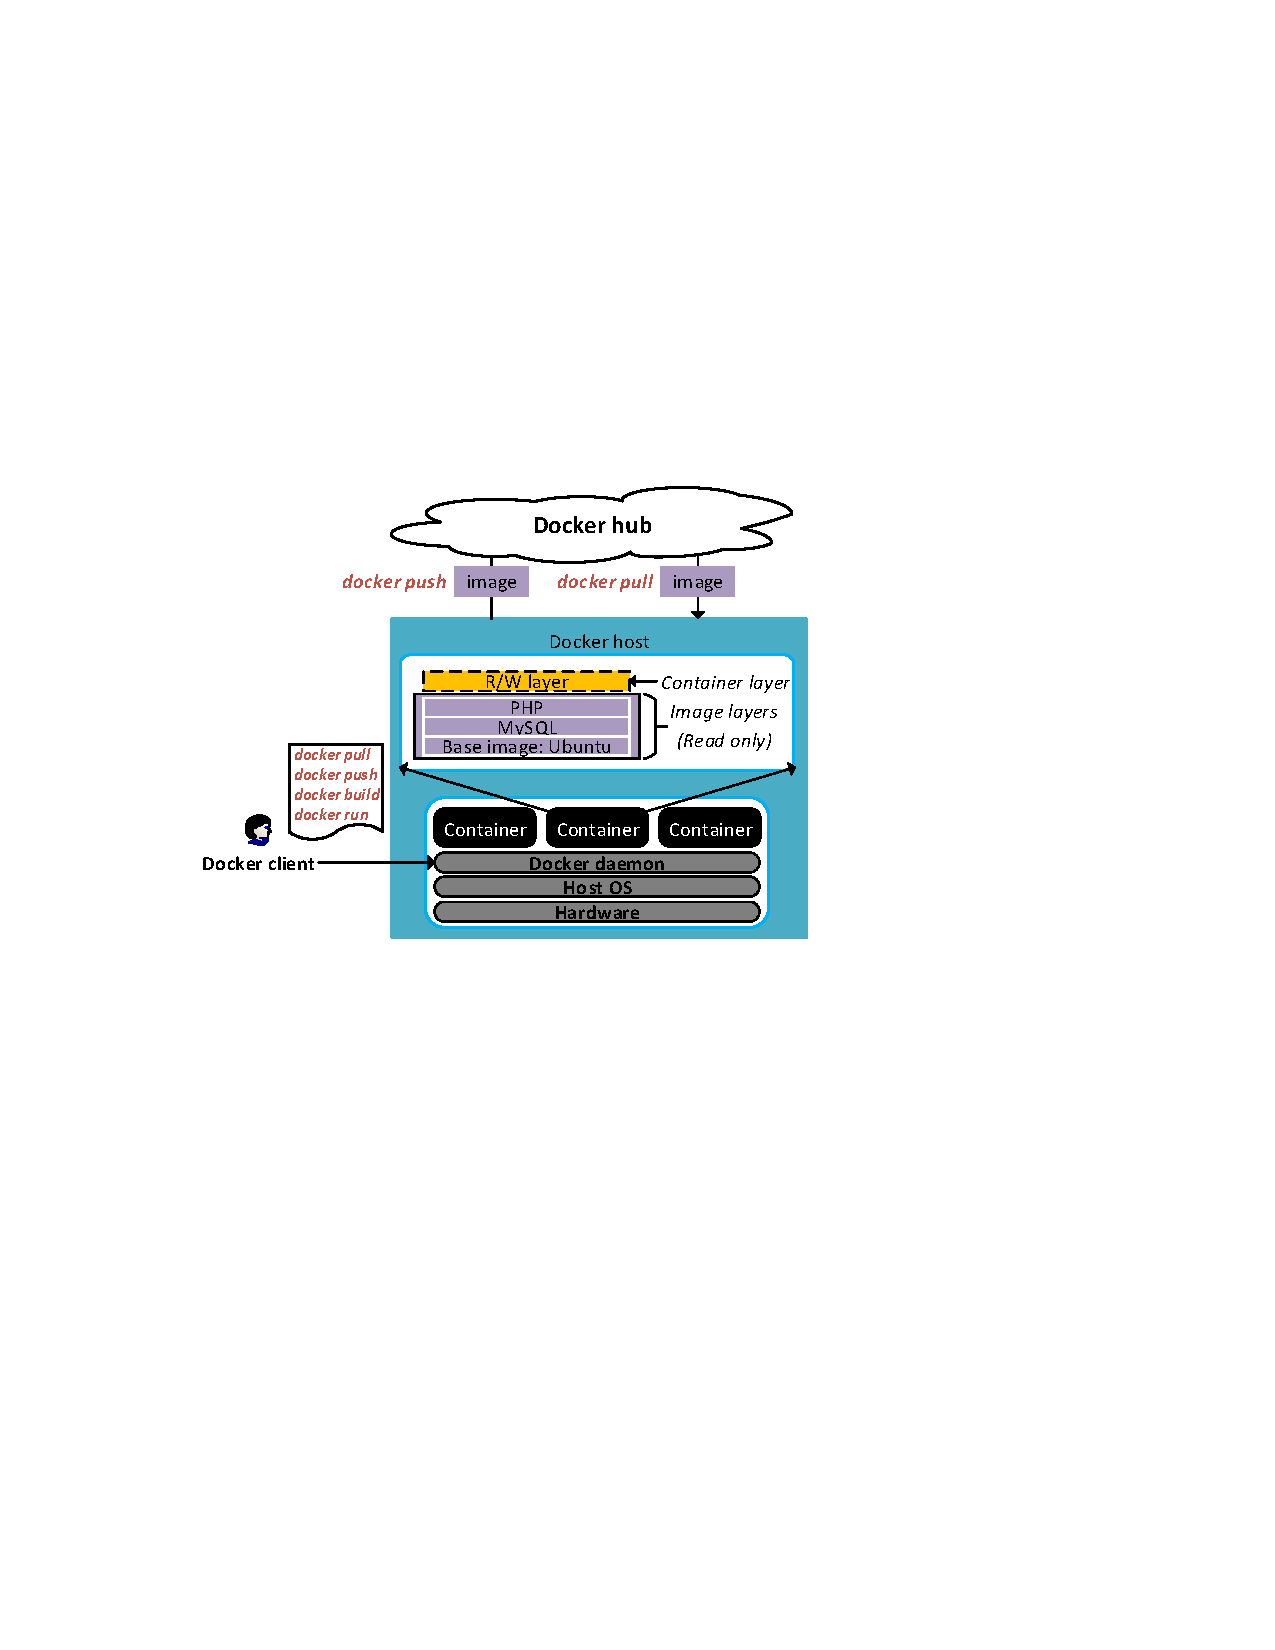
\includegraphics[width=0.5\textwidth]{graphs/fig-docker-architecture}
	\caption{Docker ecosystem
%	\lrcomment{We need to update the figure to capture
%	all the main interactions between the components and remove some unneeded
%	detail, \eg official and unofficial repositories\nancomment{addressed}}
	}
	\label{fig-docker-architecture}
\end{figure}
%
As shown in Figure~\ref{fig-docker-architecture}, a typical
Docker setup consists of three main components: 1)~\emph{client},
2)~\emph{host}, and 3)~\emph{registry}.
%
Users interact with Docker using the Docker client which, in turn,
sends commands to the Docker host.
%
Both client and host can run on the same machine.
%
Docker host runs a daemon process that implements the core logic of Docker and
is responsible for \emph{running} containers from locally available
images.
%
If a user tries to launch a container from an image that is not available
locally, the daemon \emph{pull}s the required image from the Docker registry.
%
Additionally, the daemon supports \emph{building} new images and \emph{pushing}
them to the registry.

\paragraph{Images and layers}
%
At the center of Docker is the concept of container images for packaging,
distributing, and running applications.
%
A Docker image consists of an ordered series of \emph{layers}.
%
Each Docker layer contains a subset of the files in the image and often represents a
specific component/dependency of the image, \eg a shared library.
%
Layers can be shared between two or more images if
the images depend on the same component.

Image layers are read-only.
%
When users start a container, Docker creates a new
\emph{writable layer} on top of the underlying read-only layers
(Figure~\ref{fig-docker-architecture}).
%
Any changes made to files in the image will be reflected inside the writable
layer via a copy-on-write mechanism~\cite{docker-driver-eval}.
%
This leaves layers unmodified throughout the lifetime of a container and
enables layer sharing between multiple containers spawned from the same or
different images.
%
%Docker supports multiple \emph{storage drivers} such as Aufs or Btrfs, which
%efficiently combine read-only and writable layers in a single
%namespace~\cite{docker-driver-eval}.
%
%The writable layers are deleted when the container is deleted.

%Image is represented by a \emph{manifest} which describes the various
%constituents of a Docker image, such as the target hardware platform and
%environment settings.
%%
%Moreover, the manifest contains a list of layer digests for all layers required
%by the image.


\paragraph{Registry}
%
The Docker registry is a platform for storing and sharing container images.
%
It stores images in \emph{repositories}, each containing different versions of
the same image. 
%
For each image Docker registry stores a \emph{manifest} that describes,
among other things, which layers constitute the image.
%
%The manifest is a JSON file, which contains the runtime configuration for a
%container image (\eg target platform and environment variables) and the list
%of layers which make up the image.
%
Layers are identified via a digest that is computed as a hash (SHA-256)
over the layers' uncompressed content and stored as compressed archival files.
%
%Image layers are stored as compressed archival files and image
%manifests as JSON files.
%
%\VT{What is image manifest? Need to introduce}
%
%
%Docker Hub is one of the most popular public registries, supporting both
%public and private repositories, via which users can upload, search, and
%download images~\cite{docker-hub}.
%
%In Docker Hub, the user repositories are namespaced by user name, i.e.,
%``$\langle username\rangle/\langle repository name \rangle$", while the
%official repositories, which are directly provided by Docker Inc. and partners
%are called ``$\langle repository name \rangle$".

%Modern Docker registry identifies and addresses a layer with a digest that is
%computed based on the uncompressed layer's content (e.g., SHA-256).
%
Identifying layers by their content allows the registry to store only one instance
of a layer even if it is referenced by multiple images.
%
\LR{Is that actually done across the entire registry or only within a single
user/repository? \NZ{entire registry}}
%multiple users accidentally built identical layers.
%
However, if at least one file differs in two otherwise identical layers,
the two layers are treated as different and stored separately.

\section{Methodology}
\label{sec:methodology}


%%%%%%%%%%%%%%%%%%%%%%%%%%%%%%%%%%%%%%%%%%%stats for old dataset%%%%%%%%%%%%%%%%%%%%%%%%%%%%%%%%%%%%%%%%%%%
\begin{table*}
	\centering
	\caption{Dataset summary} \label{tab-dataset-summary}
	\begin{tabular}{c|c|c|c|c|c|c}%p{0.14\textwidth}
		\hline
		% after \\: \hline or \cline{col1-col2} \cline{col3-col4} ...
		Num. of images crawled & Num. of unique images    & Num. of images downloaded  & Num. of layers downloaded \\
		\hline
		634,412                 & 457,627                 & 346,243                    & 1,763,354  \\
		\hline
		Num. of images analyzed & Num. of layers analyzed & Compressed dataset size              &  Num. of files totally \\
		\hline
		319,620                     & 1,607,533                     & 51TB                        & 117,665,791  \\
		\hline
	\end{tabular}
\end{table*}

%%%%%%%%%%%%%%%%%%%%%%%%%%%%%%%%%%%%%%%%%%%stats for new dataset%%%%%%%%%%%%%%%%%%%%%%%%%%%%%%%%%%%%%%%%%%%
%\begin{table*}
%	\centering
%	\caption{Dataset summary} \label{tab-dataset-summary}
%	\begin{tabular}{c|c|c|c|c|c|c}%p{0.14\textwidth}
%		\hline
%		% after \\: \hline or \cline{col1-col2} \cline{col3-col4} ...
%		Num. of images crawled & Num. of unique images    & Num. of images downloaded  & Num. of layers downloaded \\
%		\hline
%		634,412                 & 457,627                 & 346,243                    & 1,763,354  \\
%		\hline
%		Num. of images analyzed & Num. of layers analyzed & Compressed dataset size              &  Uncompressed dataset size \\
%		\hline
%		344,056                     & 1,748,089                     & 51TB                        & xxx  \\
%		\hline
%	\end{tabular}
%\end{table*}

In this section we describe our methodology for:
%
(1)~obtaining a representative Docker image dataset, and
%
(2)~analyzing basic and deduplication properties of the dataset.

%
\begin{figure}
	\centering
	% Requires \usepackage{graphicx}
	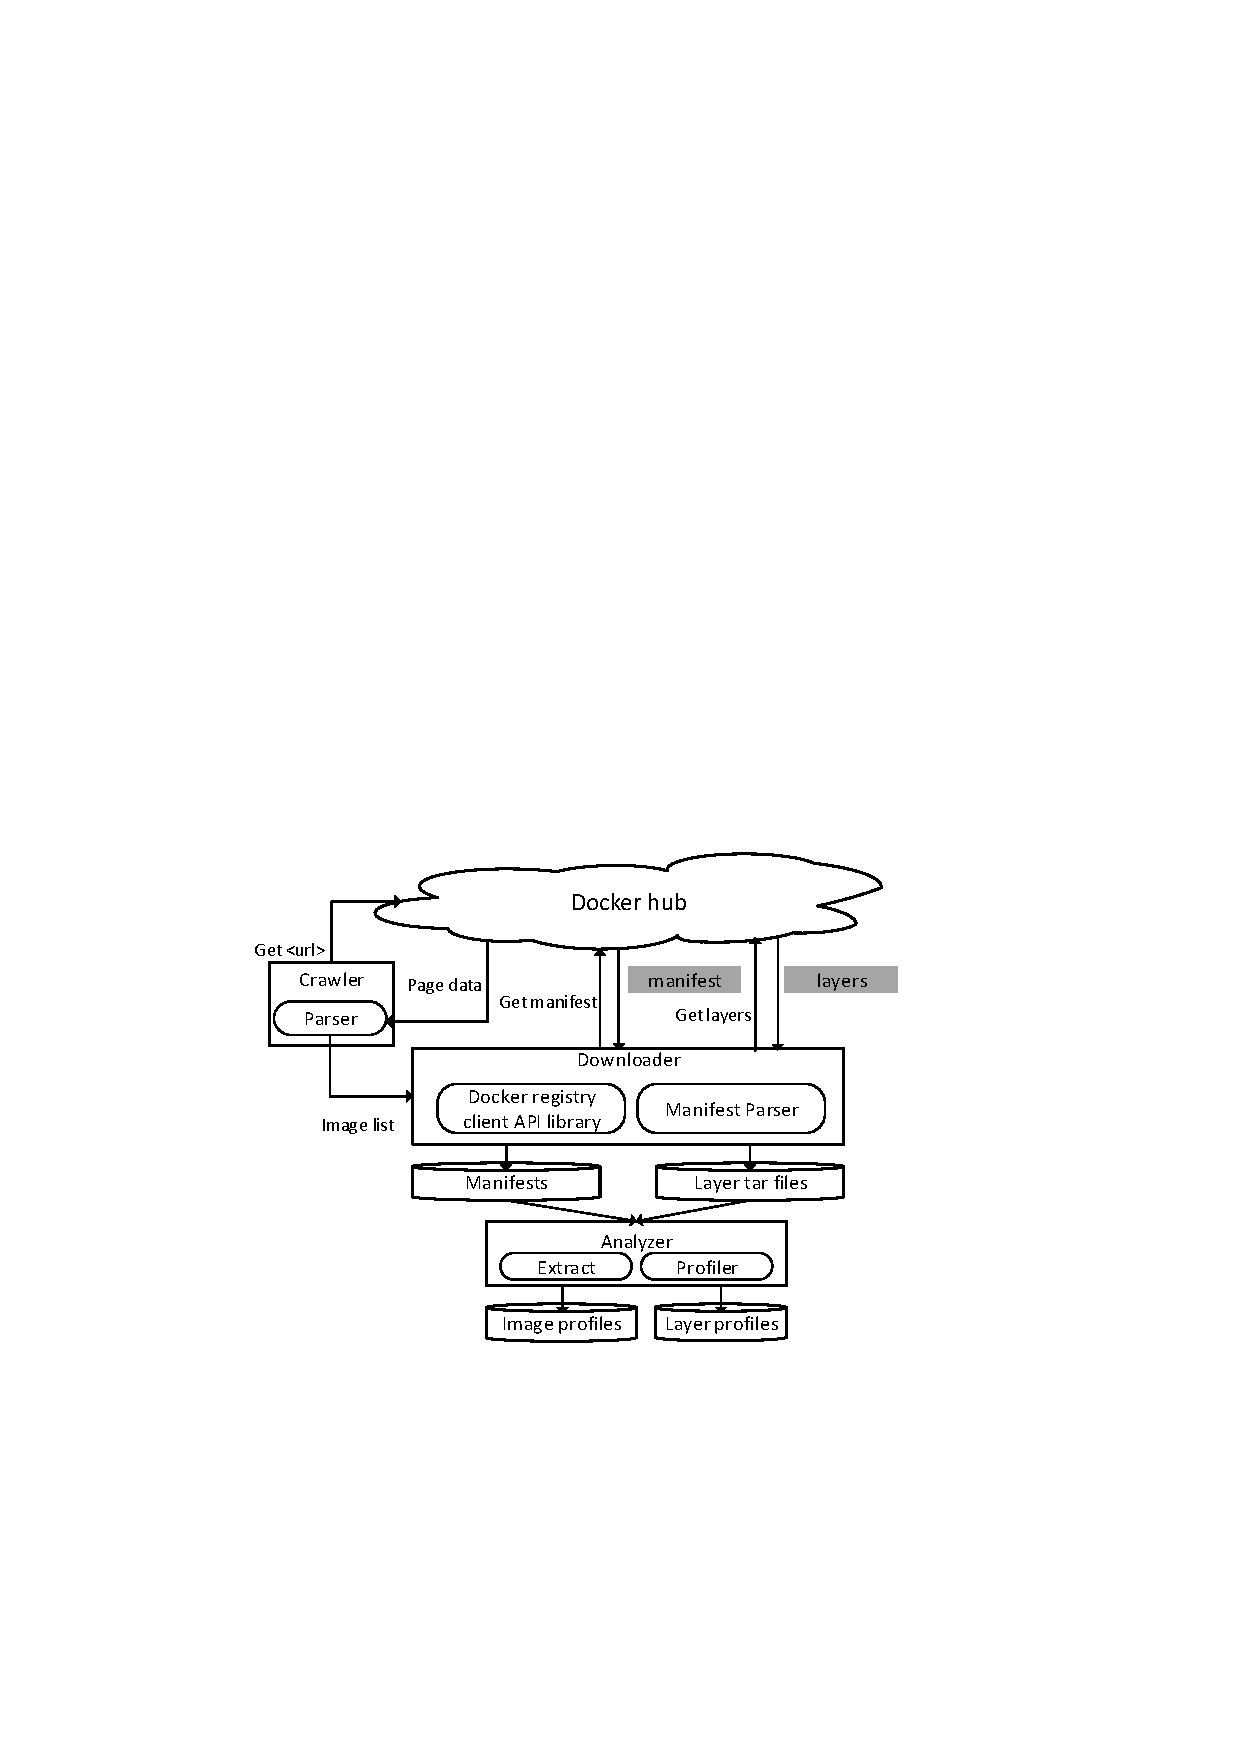
\includegraphics[width=0.5\textwidth]{graphs/fig-downloader-analyzer.pdf}\\
	\caption{Crawler, Downloader, and Analyzer
		%\vcomment{Can we add colors to this figure? Also, increase the font a bit.}
	}
	\label{fig-downloader-analyzer}
\end{figure}

\subsection{Dataset acquisition}
\label{sec:crawler}

We chose Docker Hub~\cite{docker-hub} to download a representative dataset
because (1) Docker Hub is a popular Docker registry for developers to store and
distribute Docker images, and (2) Docker Hub contains a large amount of
\emph{public} Docker images that are available for developers to download for
free.
%
We believe Docker Hub dataset is representative of other registry deployments.

To download a representative dataset from Docker Hub, web crawling is needed
because Docker Hub does not provide an API to retrieve all repository names.
%
Specifically, there are two steps: i)~crawl Docker Hub web pages to list all
repositories; ii)~download the \textit{latest} image (and referenced layers)
from each repository based on the crawler results.
%
Here, we chose latest image from each repository because (1)~the ``latest''
version is usually the newest, stable, and commonly pulled by developers;
(2)~downloading only the ``latest'' version can shorten our downloading process
since the latest images already took about 30 days to download.
%
We plan to extend our analysis to other, non-``latest'', images in the future.

\paragraph{Web crawler}

Public repositories in Docker Hub are divided into official
repositories---served by the Docker Hub partners---and non-official
repositories---provided by regular users and third-party organizations.
%
The number official repositories is less than 200, while, the majority of
repositories in Docker Hub are non-official (over 400 thousand).
%
To list non-official repositories, our crawler utilizes the Docker Hub
web-based search engine to find all available repositories.
%
As the name of non-official repositories is comprised of the user name and the
repository name separated by a ``/'', we can search for ``/'' and obtain a list
of all non-official repositories.
%
The Crawler downloads all pages from the search results and parses the web
content to build a list of all non-official repositories.
%
We ran the crawler on May 30th, 2017 and it produced a list of 634,412
repositories.
%
After removing duplicate entries (introduced by Docker Hub indexing logic), the
final repository list consists of 457,627 distinct repositories.

\paragraph{Downloader}

Instead of using the Docker client to download images, we implement our own
downloader, which calls the Docker registry API
directly~\cite{dockerregistryclient} to download manifests and image layers in
parallel.
%
Our downloader runs significantly faster than a \texttt{docker pull}-based
downloader because the latter one performs other operations besides downloading
the image, such as unpacking the layers and creating the corresponding
read-only snapshots.
%
Our downloader can download multiple images simultaneously and fetch the
individual layers of an image in parallel.
%
Layers are transferred as gzip compressed tar archives.
%
Overall, we downloaded 51~TB of data in 355,319 image manifests with 1,792,609
compressed layers. A total of 111,384 images could not be downloaded mainly because they did not have the \texttt{latest} tag. 
%
\vcomment{Say just one sentence why we did not download some images.}\nancomment{Addressed}
%
Table~\ref{tab-dataset-summary} summarizes the properties of the downloaded
dataset.

%We released both the software that we designed
%to download the images and all profiles we generated
%publicly at {\small{\url{https://elided.for.review}}}.

\subsection{Dataset analysis}

To characterize the dataset perform its redundancy analysis, we first created a
profile for each layer and image, then we performed an in-depth analysis by
using Spark~\vcomment{cite}.

\paragraph{Profiler}

For each image and each layer, profiler creates a profile in JSON format.
%
An image profile contains layer IDs, compressed size, archival size, and
compression ratio of image or layer\vcomment{what?}\nancomment{addressed}.
%
To generate a layer profile, profiler first unpacks layer tarball.
%
A layer profile consists of: (1)~layer metadata, such as layer id, compressed
size, archival size, compression ratio, directory count and file count.
%
(2)~for every file in a layer---file name, file content digest, file type, and
file size.\nancomment{add digest algori, type migic library}
%
Totally, we 1,762,639 layer profiles and 355,196 image profiles. A total of 11,130 images cannot be analyzed because their layers reported reported errors during
extraction and could not be analyzed.
%
\vcomment{Explain briefly why we did not analyze all downloaded images and
layers.}\nancomment{addressed}

\paragraph{Spark-based analyzer}

To quickly perform analysis on hundreds of thousands of profiles, we built an
8-nodes HDFS~\vcomment{cite} and Spark~\vcomment{cite} cluster.
%
We stored all the layer and image profiles in HDFS as parquet
files~\vcommnet{cite}.
%
We then performed basic and redundancy analysis using Spark SQL
module~\vcomment{cite}.
%
For example, for deduplication analysis, we first query unique file content
digests and redundant file content digests along with their repeat counts and
sizes from the layer and image parquet tables.
%
We then calculate corresponding deduplication ratios, as detailed in
Section~\vcomment{ref}.

%and investigated the following questions (RQs):  

%\paragraph{RQ1: What are the redundant ratio of layers and images?}
%
%
%\paragraph{RQ2: What are the redundant files \& why there are so many redundant files?}
%%\nancomment{how to get file type?}
%
%\paragraph{RQ3: How to reduce the redundant files?}
%\nancomment{how to prototype?}

%%%%%%%%%%%%%%%%%%%%%%%%%%%%%%%%%%%%%%%%%%%%%%%%%%%%%%%%%%%%%%%%%%%%%%%%%%%%%%
%                                                                            %
%                                OLD METHO                                   %
%                                                                            %
%%%%%%%%%%%%%%%%%%%%%%%%%%%%%%%%%%%%%%%%%%%%%%%%%%%%%%%%%%%%%%%%%%%%%%%%%%%%%%
%%\nancomment{
%%	TODO: \\
%%	1. Complete fig and table\\
%%}
%
%\lrcomment{ I think in general it would be good if we emphasize in this section, what
%was challenging about downloading all this data and how the presented approach
%overcame these challenges. \nancomment{challenges include: 1. obtaining a list of all the repositories in docker hub; 2. effectively downloading all the images. 3. indept analysis}}
%
%Our methodology consists of three steps~(Figure~\ref{fig-downloader-analyzer}):
%1)~crawl Docker Hub to list all official and nonofficial repositories;
%2)~download the latest image (and referenced layers) from each repository based
%on the crawler results; 3) unpack and analyze images and layers.
%
%%
%%
%%The first step is to massively download the Docker images from Docker registry.
%%
%%When the images are downloaded, we analyze them and calculate statistics distribution for
%%different metrics.
%%
%%The details of each step are covered in the following sections.
%%
%%\vcomment{I suggest to restructure this section simirarly to background to
%%revolve around the figure. Once you add the diagram describing our methodology
%%(like we put on the whiteboard ones), start describing components on it in the
%%order they are used: crawler, downloader, analyzer. Having two subsection:
%%``downloader'' and ``downloading images'' is confusing.
%%
%%We might want to have less deep structure also:
%%
%%3. Methodology
%%  (Figure)
%%3.1 Crawler
%%3.2 Downloader
%%3.3 Analyzer
%%}
%%
%%\nancomment{addressed}
%
%%\nancomment{
%%	figures are stored in google drive, the link is pinned in slacker;
%%	%https://drive.google.com/open?id=0B4jePsYXW6SSTTRLb0FHVXVjNUk
%%	figures/fig-docker-architecture.pdf}\\
%
%
\begin{figure}
	\centering
	% Requires \usepackage{graphicx}
	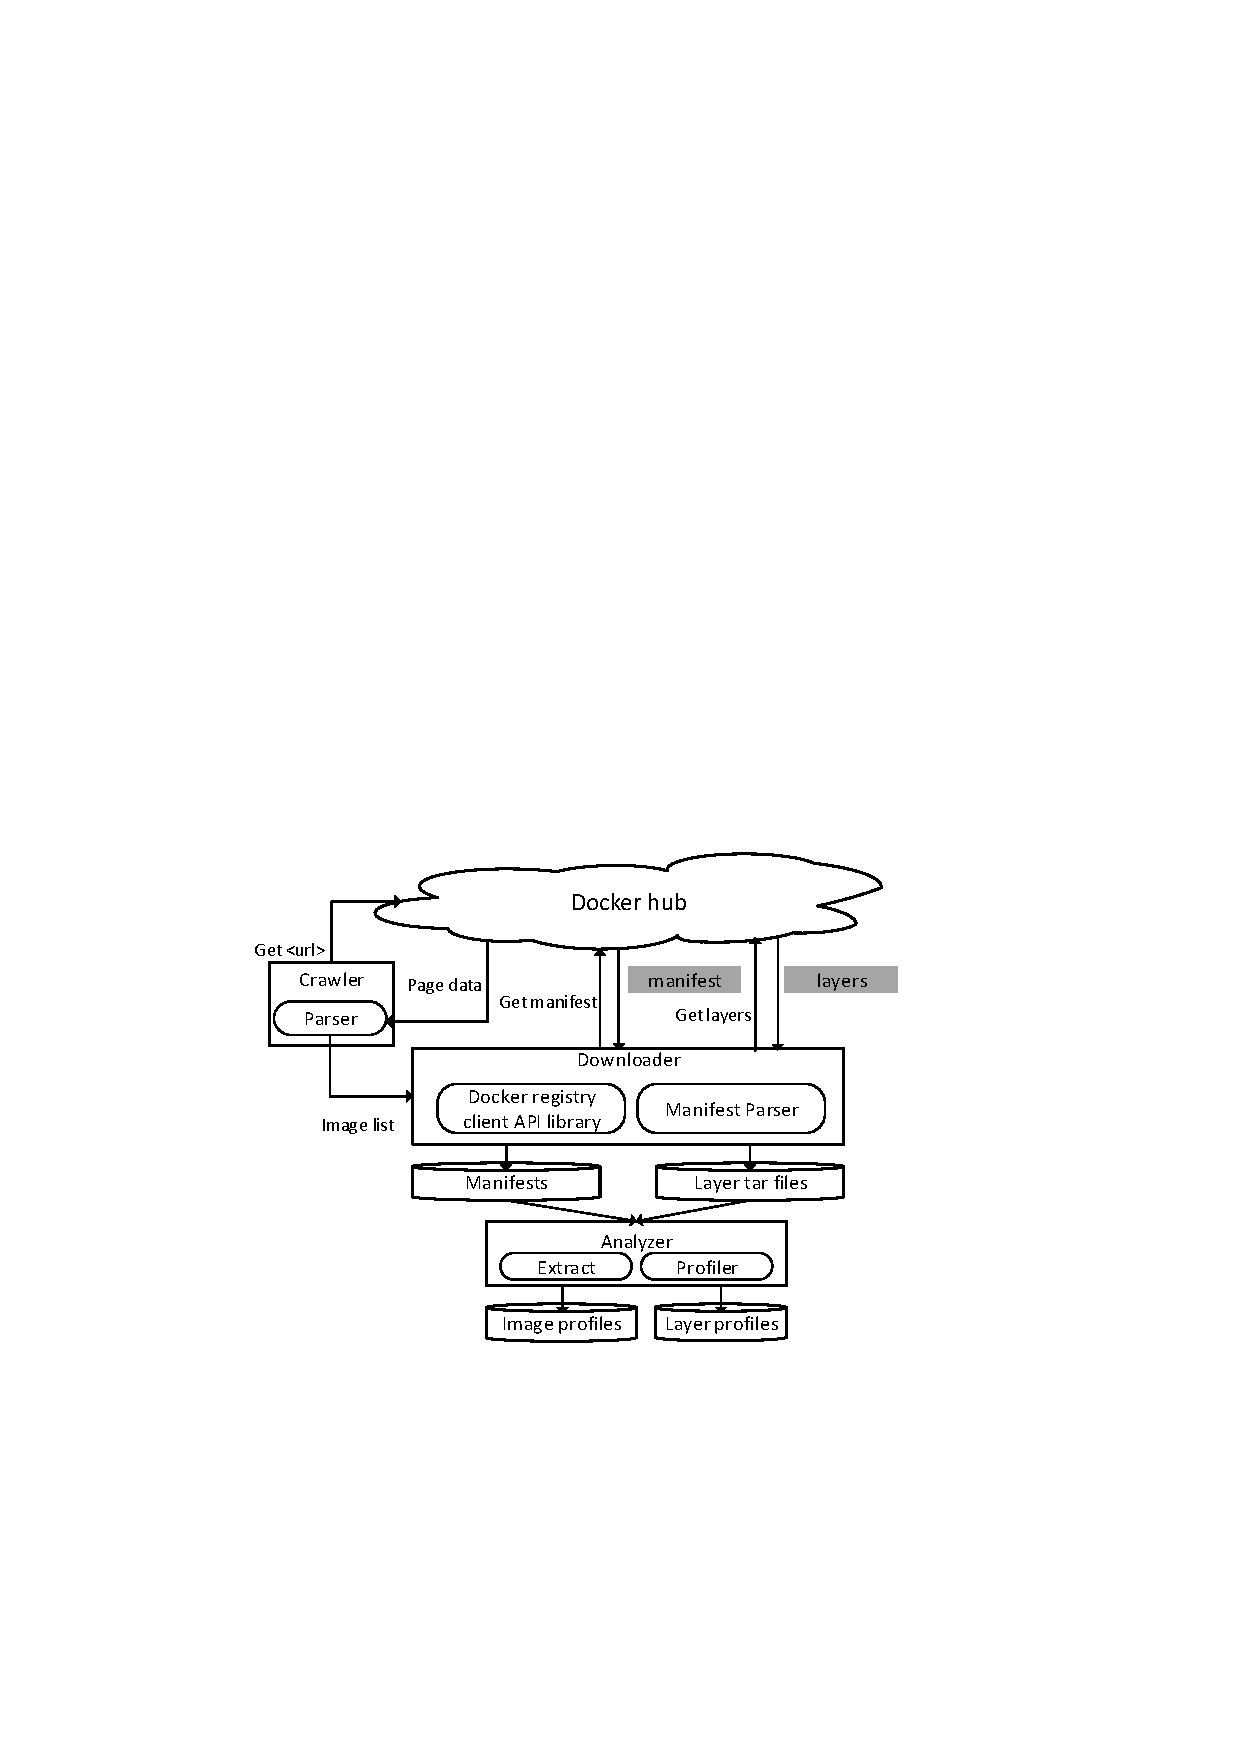
\includegraphics[width=0.5\textwidth]{graphs/fig-downloader-analyzer.pdf}\\
	\caption{Crawler, Downloader, and Analyzer
		%\vcomment{Can we add colors to this figure? Also, increase the font a bit.}
	}
	\label{fig-downloader-analyzer}
\end{figure}
%
%%how container deameon.
%%
%\subsection{Crawler}
%\label{sec:crawler}
%
%%
%To download a particular image, %or set of images (i.e., a repository)
%the name of the repository name which the image belongs to should be provided.
%The crawler is responsible
%for generating a list of repositories for the downloader.
%%as mentioned in Section~\ref{sec:docker-registry}. 
%%
%%
%%
%%\vcomment{Here and in the whole text we need to be very carefull distinguishing names 
%%of repository and image. Also discussion on image tags is missing, should be in
%%background section.}
%%\nancomment{addressed.}
%%
%Public repositories in Docker registry are divided into official
%repositories---served by the Docker Hub's partners---and non-official
%repositories---provided
%by regular users and third-party organizations.
%%, where For example, official repository Ubuntu Here is an example of the shared 
%%repository official repository Ubuntu and one of its tags. 
%%
%%A repository is a set of Docker images. A repository can be shared by pushing it to a
%%registry server. 
%%Public repositories in Docker registry can be divided into official images and non-official 
%%images.
%%
%The number official repositories is less than 200,
%% The list of official repositories
%%can be retrieved via \lrcomment{add how to list official repos}
%while, the majority
%of repositories in Docker Hub (about 400 thousands)
%are non-official.
%% (around \lrcomment{add number}).
%Listing non-official repositories requires web crawling because
%%to the best of our knowledge,
%Docker Hub does not provide an API to retrieve all repository names.
%
%Therefore, we implemented a Crawler to crawl Docker Hub and list all non-official
%repositories.
%%
%Docker Hub provides a search engine which indexes public repositories and allows
%users to search for a repository according to
%some search string. 
%%
%As the name of non-official repositories is comprised
%of the user name and the repository name separated by a ``/'',
%we can search for ``/'' and obtain a list of all non-official
%repositories.
%%``$\langle namespace\rangle/\langle repository name \rangle $", where~\textit{namespace}
%%is the user name. 
%%
%%In this case, we search for `/' and obtain a list of repositories which contains '/'.
%%
%%In other words, this method lists all the non-official public repositories in Docker Hub.
%%
%The Crawler downloads all pages from the search result.
%%
%Once web pages are downloaded, it parses the web content to build a list of
%all non-official repositories.
%
%%\lrcomment{It may be good to discuss how accurate this method is. Can we miss anything?
%%Can we get wrong results?}
%
%
%
%We ran the crawler on May 30th, 2017 and it delivered a list of 634,412 repositories.
%%
%However, the obtained list contained duplicate entries because 
%the crawling process is not atomic and some repositories have ``/'' in their description.
%%
%After removing all duplicates, the final repository list consists of 457,627
%distinct repositories. 
%%
%
%
%%
%%\vcomment{Explain why, state that it is future work.} 
%%\nancomment{addressed}
%%
%%\vcomment{I'd comment out discussion on '*'---it has low importance.}
%%\nancomment{addressed. let's comment it now and see how to deal with this issue}
%%Note that the namespace of official images is `\textit{library}'.
%%
%
%\subsection{Downloader}
%\label{sec:downloader}
%
%Docker repository is a set of images labeled with \emph{version tags}.
%%The different images in the repository are labeled with tags.
%%
%For example, \texttt{ubuntu:17.10} refers to image version \texttt{17.10} in the
%\texttt{ubuntu} repository.
%%
%If user does not provide a tag when pulling an image, 
%Docker daemon uses the \texttt{:latest} tag by default.
%For example, \texttt{docker pull ubuntu} command pulls the
%\texttt{ubuntu:latest} image.
%%
%In this work we only download images with the \texttt{:latest} tag to
%make the analysis more feasible.  We believe that the latest
%images versions represent most up-to-date state of  Docker images
%%
%and plan to analyze images with other tags in the future.
%
%
%
%%The downloader takes the list from the crawler as an input and retrieves
%%all the listed images from Docker Hub (see Figure~\ref{fig-downloader-analyzer}).
%%
%Instead of using Docker CLI to download images,
%%via the Docker Engine,
%we wrote our own downloader that calls Docker registry API directly.
%We used Docker registry client~\vcomment{insert the name, \nancomment{it is called Docker registry client}} library~\cite{dockerregistryclient} to simultaneously
%download \emph{original} manifests and image layers. \lrcomment{What does
%`original' mean here? \nancomment{without any modification}}
%%
%%\vcomment{Should we mention and cite the library that we used here?}
%%
%%\nancomment{addressed (cited in the following para)}
%%
%%
%%We decided to implement a separate downloader due to several reasons:
%%
%Our downloader runs significantly
%faster than \texttt{docker pull}-based downloader
%because the latter one performs
%operations other than downloading the
%image.
%%such as extracting
%%tar archive files and converting manifest version. 
%%
%For example, it automatically extracts each layer's tar archive file
%and creates corresponding read-only snapshot with  configured Docker storage driver.
%%and converts the manifests that are schema version 1 to schema version 2
%%(starting from Docker engine version 1.10).
%This
%not only takes considerable amount of time but also leads
%to overly high storage space utilization.
%%
%% affects
%%our results about manifest version statistics;
%%
%Furthermore, the local storage format of Docker client makes it difficult
%to analyze the contents of each layer separately.
%%Second, layer content directories are not visible for some Docker storage
%%drivers, e.g., devicemapper, which is not feasible to analyze the layer
%%content. 
%%
%%\vcomment{I think most importantly it is faster because we do not need to
%%perform extra steps that Docker client performs.}
%%\nancomment{addressed}
%%
%
%Our downloader can download multiple images simultaneously and fetch
%the individual layers of an image in parallel.
%%within each image downloading process, layers are downloaded in parallel.
%%
%%To download the original manifests and layers from Docker Hub, downloader
%%embeds a library called Docker registry client API citeXXX which only encapsulates
%%manifest and layer downloading functions in Docker engine without extracting layer
%%tarball and converting manifest version. 
%%
%%
%%\subsubsection{Downloading images}
%%
%%\vcomment{definitely need to merge this subsection with Downloader subsection.
%%See my comment for the whole section.}
%%\nancomment{addressed}
%%
%%As shown in Figure~\ref{fig-downloader-analyzer}, downloader first obtains a 
%%list of public images through crawling Docker Hub.
%%
%%Then, it starts downloading process.
%%
%%It mainly downloads two components: manifest and individual layer files. 
%The process consists of two steps.
%%
%First, fetching the manifest by sending a \texttt{GET} request to
%$/v2/\langle name \rangle/manifests/\langle reference \rangle$,
%where~\textit{name} refers to
%$\langle namespace\rangle/\langle repository name \rangle$
%and \textit{reference} is typically a version $\langle tag \rangle$.
%%
%%
%%\lrcomment{Are the following 4 sentences needed?}
%%Note that the~\textit{namespace} of official is~\textit{library}.
%%
%%The reference can include a tag or digest.
%%
%%Note that currently we only downloaded the images with~\textit{latest} tag to shorten
%%the downloading process. In the future, we will download all the images with different tags.
%%
%%As discussed in Section~\ref{xxx}, manifest consist of multiple layer digests.
%%
%%Note that Schema 2 versioned manifest also contains a config file digest.
%%\vcomment{I believe we never explained what is config file. We need to discuss in
%%in background section.}
%%\lrcomment{Do we use config files in the analysis? If they contain the command
%%to run in the container, I think that could give us some interesting insights into
%%how people use containers.}
%%
%Second, once the manifest is downloaded, the downloader uses the layer digests to
%download individual layers
%%(including the config file for Schema 2 versioned manifest)
%by sending $GET$ request to $/v2/\langle name \rangle/blobs/\langle digest \rangle$.
%\textit{Name}, as for manifests,
%refers to $\langle namespace\rangle/\langle repository name \rangle$
%while~\textit{digest} refers to the layer digest.
%%or config file digest.
%Layers are transferred as gzip compressed tar archives.
%%\vcomment{What compression is used?}
%%\nancomment{addressed}
%
%%
%%\vcomment{I believe different parts of this section belong to different
%%	earlier parts: some to crawler, some to downloader.}
%%\nancomment{addressed}
%%
%
%
%The whole downloading process took around 30 days.
%%
%Overall, we downloaded 51~TB of data in 355,319 image manifests with 1,792,609
%compressed layers.
%%
%A total of 111,384 images could not be downloaded due to three reasons.
%%
%First, 5\% of the images required authentication and
%second, 87\% of the images did not have the \texttt{latest} tag.
%Third, 8\% of the images contains layers that cannot be downloaded.
%% 0.05189255189	0.8666056166 0.0815018315
%%As we discussed in Section~\ref{sec:crawler}, we only downloaded the \texttt{latest}
%%version of an image to shorten the downloading process.
%Table~\ref{tab-dataset-summary} summarizes the properties of downloaded
%dataset.
%
%%\nancomment{2. TODO: add a table discribe:\\
%%	how many images, duplicate ratio\\
%%	how many cannot download, (removed, no latest)\\
%%	how many layers, config, manifest\\
%%	dataset}
%
%%\subsubsection{Docker image dataset statistics}
%
%
%
%%The reason probably is that Docker Hub adjusted websites'order or modified the
%%websites because of the increasing of Docker images during our crawling process.
%%Our crawler has a unavoidable delay between each HTTP requst and HTTP response. 
%%So it couldn't reflect the websites'order or website content changes. Another
%%reason is that search engine lists duplicated images 
%
%%Overall, we downloaded XXX image with XXX layers. Table~\ref{XXX} summaries
%%the statistics of Docker image dataset we downloaded. Then, we profiled the
%%layers, config files, and manifests we downloaded and calculated the statistic
%%distribution for different metrics. 
%
%%Some embedded literal typset code might 
%%look like the following :
%%
%%{\tt \small
%%\begin{verbatim}
%%int wrap_fact(ClientData clientData,
%%              Tcl_Interp *interp,
%%              int argc, char *argv[]) {
%%    int result;
%%    int arg0;
%%    if (argc != 2) {
%%        interp->result = "wrong # args";
%%        return TCL_ERROR;
%%    }
%%    arg0 = atoi(argv[1]);
%%    result = fact(arg0);
%%    sprintf(interp->result,"%d",result);
%%    return TCL_OK;
%%}
%%\end{verbatim}
%%}
%%
%%Now we're going to cite somebody.  Watch for the cite tag.
%%Here it comes~\cite{Chaum1981,Diffie1976}.  The tilde character (\~{})
%%in the source means a non-breaking space.  This way, your reference will
%%always be attached to the word that preceded it, instead of going to the
%%next line.
%
%\begin{table*}
%	\centering
%	\caption{Dataset summary} \label{tab-dataset-summary}
%	\begin{tabular}{c|c|c|c|c|c|c}%p{0.14\textwidth}
%		\hline
%		% after \\: \hline or \cline{col1-col2} \cline{col3-col4} ...
%		Num. of images crawled & Num. of unique images    & Num. of images downloaded  & Num. of layers downloaded \\
%		\hline
%		634,412                 & 457,627                 & 346,243                    & 1,763,354  \\
%		\hline
%		Num. of images analyzed & Num. of layers analyzed & Compressed dataset size              &  Uncompressed dataset size \\
%		\hline
%		344,056                     & 1,748,089                     & 51TB                        & xxx  \\
%		\hline
%	\end{tabular}
%\end{table*}
%
%\subsection{Analyzer}
%\label{sec:analyzer}
%
%The analyzer analyzes extracts downloaded layers
%and analyzes them along with image manifests.
%It creates two types of profiles for each image:
%an image profile and individual layer profiles.
%Each profile contains different metrics for the whole image and
%its individual layers, respectively.
%Profiles are stored in JSON format.
%
%
%%
%%\vcomment{I think we do not need to discuss any metrics above, as you
%%discuss them below in corresponding subsections.}
%%\nancomment{addressed}
%%
%
%\paragraph{Layer profile.}
%
%Layers are downloaded as compressed tar archive files.
%%
%To produce the layer profile, the analyzer first decompresses and extracts each
%layer tarball to a layer directory.
%%
%Then, it recursively traverses each subdirectory and obtains
%the metadata information for each subdirectory.
%
%The layer profile contains metadata about the layer, its directories,
%and files: 
%
%\{
%layer digest; 
%Archived layer size (ALS); 
%Sum of containing file sizes (FLS); 
%Compressed layer size (CLS); 
%ALS-to-CLS (compression ratio);
%FSL-to-CLS (compression ratio);
%Directory count;
%File count;
%Layer directory depth;
%\}
%
%\{
%Directory name;
%Directory depth;
%File count;
%Directory size;
%\}
%
%\{
%File name;
%File digest;
%File type;
%File size;
%\}
%
%\begin{compactitemize}
%	\item XXX
%	\item XXX
%	\item XXX
%	\item XXX
%\end{compactitemize}
%
%%file count while directory metadata covers directory depth and size
%%and file metadata includes size and type. The full set of metrics
%%covered by the layer profile is shown in Table~\ref{xxx}.
%
%
%%Each layer profile contains
%%layer metadata information, such as layer size and file count; and
%%directory metadata information for each subdirectory, such as directory
%%depth and directory size; and file metadata information for each file,
%%such as file size and file type.
%%
%%\vcomment{I'm not sure what figure we want here. I think a table might suffice.}
%%\nancomment{addressed}
%%\nancomment{3. TODO: 
%%	add a fig: discribe all layer metadata, config metadata, and manifest metadata structure} 
%%
%%\nancomment{4. TODO: 
%%	add a table\\
%%	layer tarball format statistics, tar, compressed, non compressed\\
%%	config statistics, txt, json\\
%%	manifest statistics, txt, json}
%\vcomment{Instead of the table, let's us the itemized list above for now, \nancomment{already add table 1. and we dont need to list metrics here since we present them in results}}
%
%
%\paragraph{Image profile.}
%
%To create the image profile, the analyzer parses the manifest
%and obtains the configuration information such as OS and architecture.
%Further, once individual layers are analyzed, the analyzer can build the whole image
%profile by including pointers to its layer profiles. In total, image profile includes
%the following information:
%\{
%Image name; 
%Archived Image size (AIS); 
%Sum of containing file sizes (FIS); 
%Compressed image size (CIS); 
%ALS-to-CLS (compression ratio);
%FSL-to-CLS (compression ratio);
%Directory count;
%File count;
%\}
%
%\begin{compactitemize}
%	\item XXX
%	\item XXX
%	\item XXX
%	\item XXX
%\end{compactitemize}
%
%% image metadata information,
%%such as image pull count and layer count, and image configuration
%%information, such as OS version and architecture. All metrics
%%in the image profile are shown in Table~\ref{xxx}.
%
%%Note that schema version 2 manifests store configuration information in a
%%config file as discussed in Section~\ref{sec-image-layers}.
%%\lrcomment{I think we removed the part about different manifest versions from
%%the background, should add it back.}
%%
%%As shown in table~\ref{xxx}, \gap of manifests are Schema version 2 while the
%%rest are Schema version 1. 
%
%%
%%
%%While layer profile
%%contains layer metadata information, such as layer size and file count;
%%and directory metadata information for each subdirectory, such as directory
%%depth and directory size; and file metadata information for each file, such
%%as file size and file type.
%%
%%Table~\ref{xxx} summaries the layer archive file, config file, and manifest
%%statistics.
%
%
%%\vcomment{This section (and some other places) contain a lot of ``etc.''. The
%%general rul of thumb never to ue etc. in a scientific paper. Instead,
%%say: "e.g.,", or "for example," or "for instance"}
%%\nancomment{addressed}
%%\subsubsection{Config profile}
%


\section{Results}

\nancomment{
	figures are stored in google drive, the link is pinned in slacker;
	%https://drive.google.com/open?id=0B4jePsYXW6SSTTRLb0FHVXVjNUk
	figures/*.pdf}\\

\subsection{Image}

\subsubsection{Growth  of images at docker registry}

%1. Fig: The total number of images increases from May 30th to Sept. XXX (May 30th - July 11th)(July 11th - Sept. 1)
%!!!!!replace image with repositories.
Figure~\ref{fig_image_growth} show the total number of images in Docker hub increases from May 30th to Sept. 17th 2017. As discussed in~\cite{XXX}, Crawler searched for `/' by using Docker hub search engine, crawled the web page, and obtained the totoal number of non-official public repositories in Docker hub each day. By summing both official image count and non-official image count, we got the total number of images in Docker hub each day. Figure~\ref{fig_image_growth_first} shows the total number of images in Docker hub each day from May 30th to July 11th. The total number of images increased from xxx to xxx, with almost 1,300 images created per day.

\begin{figure}
  \centering
  % Requires \usepackage{graphicx}
  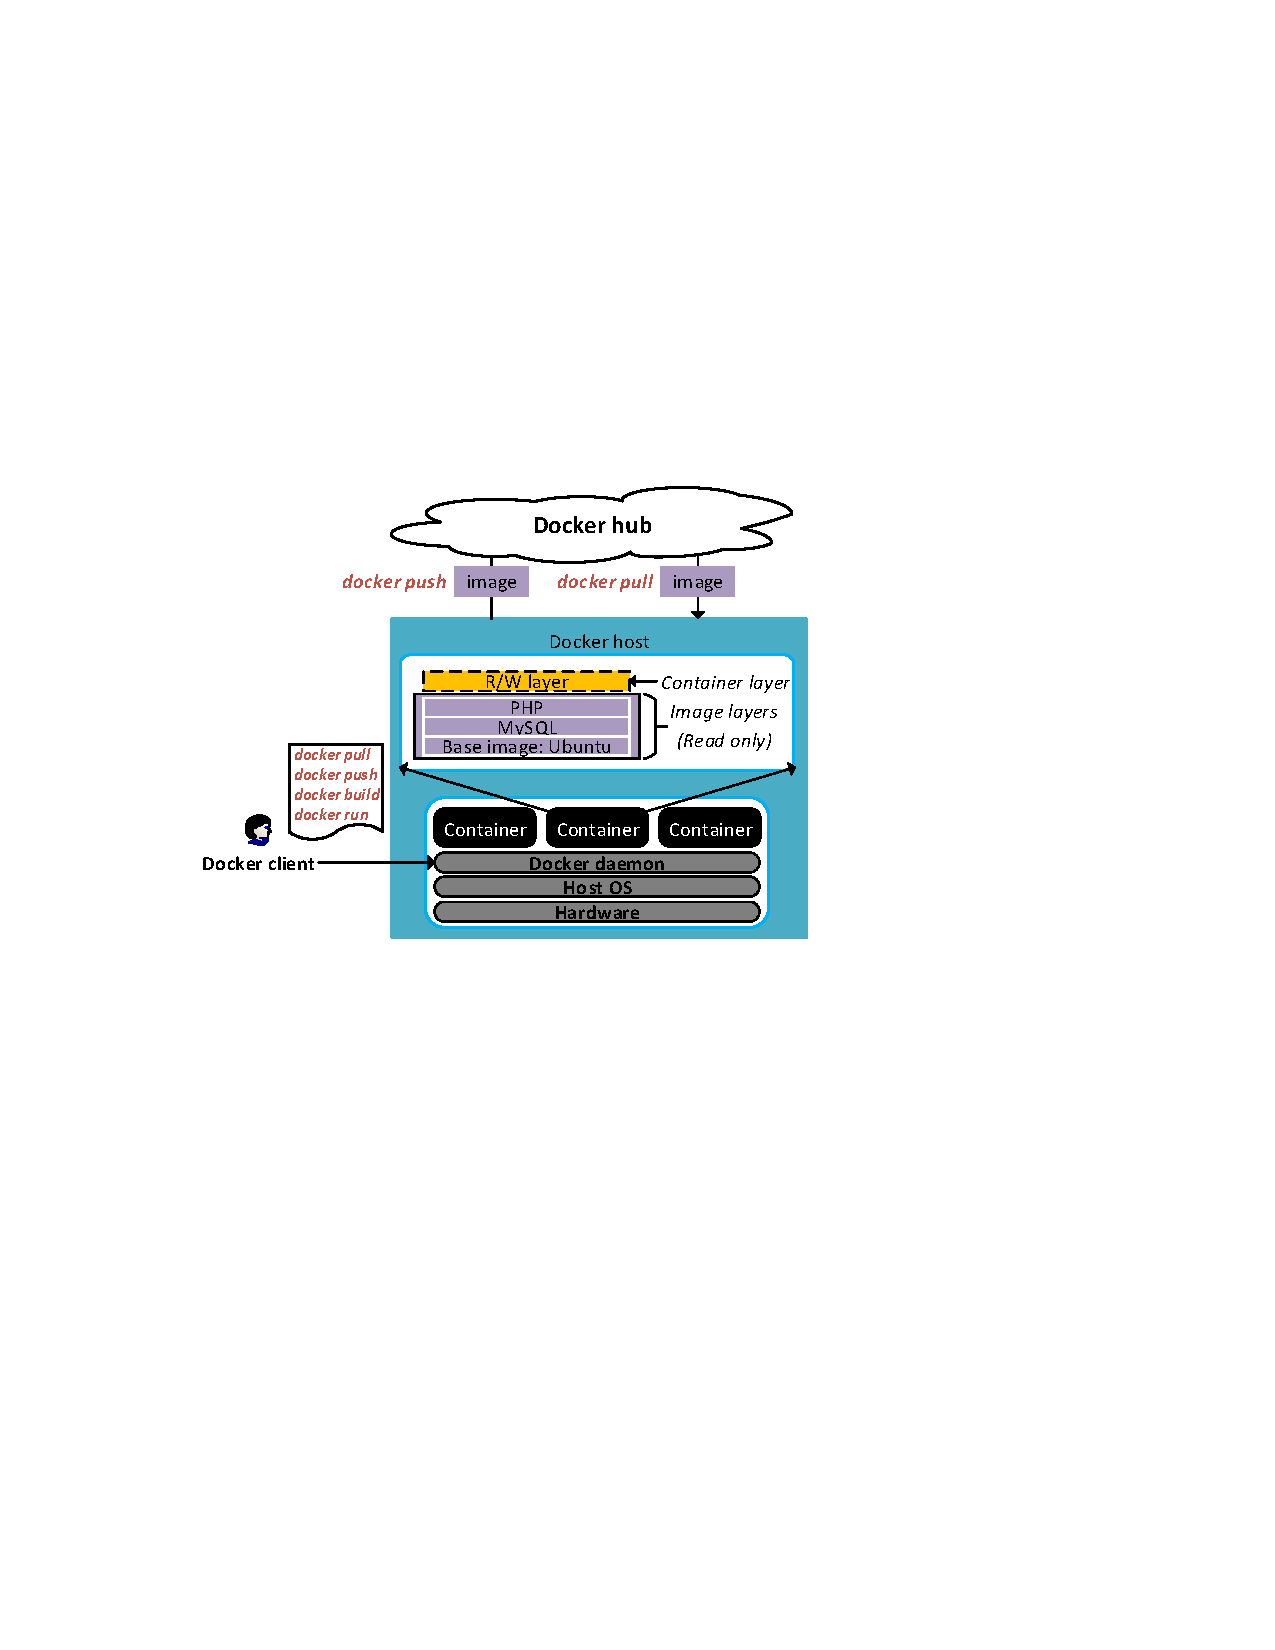
\includegraphics[width=0.45\textwidth]{graphs/fig-docker-architecture}\\
  \caption{Total number of images in Docker hub from May 30th to Sept. XXX}\label{fig_image_growth}
\end{figure}

A interesting observation is that Crawler can get a similar list of images if we replace `/' with `*'. Note that from 5/30/2017-7/11/2017, Crawler used above method to obtain the total amount of images in Docker Hub. But after 7/11/2017, the Docker Hub removed the index of `/'. Thus, currently we search for `*' instead of `/' to obtain a list of non-official public images. As shown in figure~\ref{fig_image_growth_second}, the total number of images increased from xxx to xxx, with almost xxxx images created per day.

\subsubsection{Image popularity distribution}

\nancomment{TODO: 1. Fig: The avg. number of images pulled per day from May 30th to Sept. 1}

%2. Fig: The total number of images pulled by May 30th.
Figure~\ref{fig_pull_cnt_total} shows the image popularity distribution. The x-axies show the total number of pull count for each image ranges from 0 to 250. The blue line shows the cumulative distribution of total number of pull count per image while the red line shows the frequency distribution of total number of pull count per image. 85\% of the images are pulled than 250 totally. The greatest pull count is xxx which is official image~\textit{nginx}. About 12,000 has a pull count of ~xxx.

\subsubsection{Image size distribution}

%1. Fig: Image compression size as the sum of its gzip compressed layer size.
%56\%
Figure~\ref{fig_image_size_compression} shows the image compression size distribution. The x-axies shows the image compression size which is the sum of its compressed layer size. The blue line shows the cumulative distribution of image compression size. 56\% of images are less than 50 MB. xxx of images are less than xxx MB. The biggest image is xxx GB while around 120,000 of images are less than ~2 MB. We can conclude that most of the images in Docker hub are small images, less than xxx MB.

2. Fig: Image Decompressed size as the sum of its layer decompression size.

Figure~\ref{fig_image_size_decompression}

\subsubsection{Compression rate distribution}

1. Fig: Compression ratio as the sum of its layer decompression size divided by the sum of its gzip compressed layer size.

\subsubsection{Layer count distribution}

1. Fig: Layer count distribution.

\subsubsection{Repeat layer count distribution}

1. Fig: Repeat layer count distribution.

\subsubsection{File count distribution}

1. Fig: File count distribution.

\subsubsection{Other metrics, exectution envirnoment}

\subsection{Layer}

\subsubsection{Layer size distribution}

1. Fig: Layer compression size
2. Fig: Layer Decompressed size

\subsubsection{Compression rate distribution}

1. Fig: Compression ration as the layer decompression size divided by the gzip compressed layer size.

\subsubsection{Layer depth distribution}

1. Fig: Layer depth

\subsubsection{File count distribution}

1. Fig: File count distribution.

\subsubsection{Directory count distribution}

1. Fig: Directory count distribution.

\subsubsection{Layer directory depth distribution}

1. Fig: Layer directory depth distribution.

\subsubsection{Other metrics, layer age}

\subsection{File}

\subsubsection{File count distribution}

\subsubsection{File size distribution}

\subsubsection{File type distribution}

\subsubsection{Repeat file count distribution}

\section{Related Work}
\label{sec:related}

%?: ~\cite{7158965}.
%?: ~\cite{dockerbook}.
%?: ~\cite{5655241} - dedup of containers?
%Due to its increasing popularity, Docker has recently received increased
%attention from the research community.

A number of studies investigated various dimensions of Docker storage
performance ranging from graph driver performance~\cite{slacker,docker-driver-eval,improve-cow-container-drivers}, to registry workload and image analysis~\cite{dockerworkload,dedupanalysis}
and better image management~\cite{shifter,exoclones}. However, none
of them provide deduplication capabilities for the registry.

Skourtis \etal~\cite{skourtis2019carving} proposed to reduce registry storage utilization by
restructuring layers to maximize their overlap. However, they change
the existing structure of images whereas \sysname leaves images unchanged.
%
%Many studies focus on reducing the size of Docker
%images~\cite{rastogi2017cimplifier,gschwind2017optimizing} to reduce image pulling time.
%
%DockerSlim~\cite{dockerslim} is an effective tool to minify a single image.

There is one community proposal to add file-level deduplication to container
images~\cite{Krohmer-proposal}, but doesn't provide a detailed design or performance
analysis.
%https://gist.github.com/devkid/5249ea4c88aab4c7bff1b34c955c1980#file-readme-md
%However, neither of these approaches provide a performance evaluation.
%\Ali{Slacker does provide performanve evaluation. Perhaps, we can say that none of these papers
%provide registry level deduplication and performance evaluation to quantify deduplication
%overhead.}
%
There is other work aimed at reducing image sizes to improve pulling time and 
storage use~\cite{cntr,rastogi2017cimplifier,gschwind2017optimizing,dockerslim}. 
%
These methods are orthogonal to our approach and can be used  with \sysname.
%
%Harter \etal~\cite{slacker} studied 57 images from Docker Hub for a variety of metrics
%but not for data redundancy.
%The authors used the results from their study to derive a benchmark to evaluate
%the push, pull, and run performance of Docker graph drivers based on the studied
%images. Compared to Slacker, our analysis focuses on the entire Docker Hub dataset.
%
%Cito \etal~\cite{cito2017empirical} studied 70,000
%Dockerfiles and focused on the image build process not its contents.
%of Docker ecosystem with a focus on prevalent quality issues, and the evolution of Docker 
%files based on a data set of 70,000 Docker files.
%However, their study did not focus on actual image data.
%
%Shu \etal~\cite{dockervulnerabile} studied the security vulnerabilities in Docker Hub
%for 356,218 images.
%
%Anwar \etal~\cite{dockerworkload} performed a detailed analysis
%of an IBM Docker registry workload but not the dataset.
%
% and found there is a strong need for more
%automated and systematic methods of applying security updates to Docker images. While
%the amount of images is similar compared to our study, Shu \etal focused on a subset
%of 100,000 repositories and different image tags in these repositories.
%
%Dockerfinder~\cite{dockerfinder} is a microservice-based prototype that allows searching
%for images based on  multiple attributes, e.g., image name, image size, or supported software 
%distributions. It also crawls images from remote Docker registry but the authors do
%not provide a detailed description of their crawling mechanism.
%
%Bhimani~\cite{dockerssd} \etal characterized the performance of persistent storage options
%for I/O intensive containerized applications with NVMe SSDs.
%
%Data deduplication is a well
%explored and widely applied technique~\cite{2009-sparse_indexing_inline_dedup_using_sampling-fast,
%2001-low_bandwidth_network_fs-sosp,
%2012-idedup-fast,
%tarasov2014dmdedup,
%2008-avoid_disk_bottleneck_data_domain_dedupfs-fast}.
%
%A number of studies which focus on
%real-world datasets~\cite{2009-dedup_effectiveness_on_vm_disk_images-systor,
%2012-data_reduction_in_primary_storage-systor,
%2012-hpc_practical_dedup_study-sc,
%2013-charact_increment_changes_data_protect-atc,
%msst16dedup-study,
%2012-charact_backup_workloads-fast,
%2013-charact_dedup_effic_big_data-iiswc}
% can be complementary to our approach.
%but to the best of our knowledge, we are the first to analyze a large-scale Docker
%registry dataset for its deduplication potential.
%and propose to apply deduplication to it.

Deduplication in cloud storage has been investigated for decades, particularly for virtual machine
images~\cite{zhou2013characterizing,srinivasan2012idedup,jin2009effectiveness}.
%
For instance, Jayaram~\etal~\cite{jayaram2011empirical} studied 525 images
from a production IaaS cloud and detected similarities. 
 %...because current hypervisor-based virtualization techniques do not support
 %block sharing between virtual disk images, instead relying on techniques such
 %as overlays to build multiple VMs from a single "base" image, similar with
 %Docker images.
 \sysname is different as it focuses on container images and hence, can exploit
 knowledge about files inside the image to optimize the deduplication ratio.
 
Beside virtual machine images, many studies also focused on primary and backup data
deduplication~\cite{tarasov2014dmdedup,muthitacharoen2001low,lu2012insights,2009-sparse_indexing_inline_dedup_using_sampling-fast,2013-charact_increment_changes_data_protect-atc,wallace2012characteristics,zhu2008avoiding}
and show the effectiveness of file- and sub-file-level
deduplication~\cite{2012-hpc_practical_dedup_study-sc,msst16dedup-study}.
%
\sysname utilizes file-level deduplication but is specifically designed for Docker registries,
which allows it leverage image and workload information to reduce deduplication overhead.
%
%\Ali{Id whole-file deduplication a term? If not we should stick with file-level deduplication.}


The performance of restoring the original data post-deduplication is as important as the deduplication ratio  even for backup systems~\cite{lillibridge2013improving}.
%\Ali{What is restoring performance?}
%\Subil{reworded. is this better?}
%
To improve the restoring latency, multiple optimizations are such as caching, prefetching, exploiting
historical information and temporal trends, data locality etc. are evaluated~\cite{fu2014accelerating,fu2015design,fu2011aa}. 
%
\sysname combines several of these optimizations in its design to provide efficient
image deduplication.
%
%All these optimization techniques inspire our design.
%\Ali{Related work needs to be expanded.}
%Most existing cloud storage providers employ data
%deduplication techniques to eliminate redundant data, same data stored more
%than once.

%Deduplication techniques significantly reduce storage needs and therefore
%reduce storage costs and improve storage efficiency.

%Data deduplication works by storing duplicate data chunks only once, keeping
%only the unique data chunks. 
%
%Current cloud providers deploy a cross-user client-side fixed-size-chunk-level
%data deduplication that delivers the highest deduplication
%gain~\cite{pooranian2018rare}.
%
%These approaches maximize the benefit of deduplication: The cross-user data
%deduplication treats cloud storage as a pool shared by all the cloud users,
%because the potential for data deduplication is the highest as the probability
%for redundancies and duplicates is higher the more inclusive the shared pool.
%
%The fixed-size-chunk-level specifies that a fixed-size chunk is the unit for
%checking for duplicates on cloud storage.
%
%Google cloud and AWS employ StorReduce, a deduplication software that performs
%in-line data deduplication transparently and resides between the client's
%application and the hosting cloud storage.
%
%StorReduce provide 80-97\% storage and bandwidth reduction to the cloud
%providers~\cite{StorReduce_google}.


%Unlike our study, their analysis
%is focused on the execution of containers rather than on their storage at the registry side.

%\textbf{Analysis on file systems}:
%File system contents have been widely studied in different operating system environments.
%Douceur and Bolosky collected and analyzed over ten-thousand Windows file
%systems~\cite{largefscontent}. They found that the size of file and directory are fairly
%consistent across file systems, but file lifetimes and file-name extensions vary based on
%the job function of the users. 
%Agrawal, Bolosky, Douceur, and Lorch collected and analyzed a five-year file-system metadata
%over 60,000 Windows file systems, and presented the temporal trends relating to file size,
%file type, and directory size~\cite{fiveyearfsmetadata}.
%Sienknecht, Friedrich, Martinka, Friedenbach collected file system data from UNIX systems
%based on a dataset of 46 systems, 267 file systems, 151,000 directories and 2,300,000 files
%and found small files dominate in count~\cite{distributedatainfs}.
%%Traeger, Zadok, Joukov, and Wright surveyed 415 file system and storage benchmarks from
%106 recent papers~\cite{xxx}.  

\section{Conclusion}
\label{sec:conclusion}
%\NZ{put in background or intro, conclusion, discussion?}
This paper presents \sysname~that integrates caching and deduplication with the Docker registry to
improve its performance and to decrease the backend storage capacity requirement. 
%The layer buffer holds hot layers that belong to active users.
%To improve the capacity limitation of the main memory cache, we utilize flash memory to store unique files since it offers fast random read access.
%The utilization of flash memory to store unique files not only mitigates the capacity limitation of the main memory cache, it also offers fast random read accesses.
% a on a distributed flash-based store.  \\
Moreover, we proposed a two-tier heterogeneous cache architecture to efficiently improve cache space 
utilization. We utilize the user behavior for the cache replacement algorithm to improve cache hit ratio.


\section{Discussion}
\label{sec:discussion}
In this section, we present some issues or concerns about~\sysname~and additional optimizations to help speed up~\sysname:
\paragraph{Further utilize user behavior pattern to accurately predict layer access pattern}
We observed that although half of the users have only one repository with a few layers, there are some users who own many layers. 
For future work, we will focus on precisely predicting which layers will be accessed by active users and prefetch them in the cache for later accesses.
We also observed that 

%\paragraph{How many more "layers" can fit in file cache compared with naively storing layers in file cache}
%\paragraph{Can we do client-side deduplication to remove duplicates}
\paragraph{Docker client-side deduplication: viability and implications}
Client-side deduplication affects the container runtime. 
Because performing inline file-level deduplication on the Docker client side requires intensive file 
fingerprint calculations and file fingerprint lookup, which will slow down container runtime performance.
For future work, we will offload client-side deduplication to server-side, meaning that the 
Docker client doesn't need to do deduplication because
it can push all its created images to the registry and the registry eliminates duplicate files for the client. 
In this case, Docker clients use the registry as a washing machine to launder duplicate files in their local file systems without performance overhead.


%
%Data deduplication has proven itself as a highly effective technique for
%eliminating data redundancy.
%%
%In spite of being successfully applied to numerous real datasets, deduplication
%bypassed the promising area of Docker images.
%%
%In this paper, we propose to fix this striking omission.
%%
%We analyzed over 1.7 million real-world Docker image layers and identified that
%file-level deduplication can eliminate 96.8\% of the files resulting in
%a capacity-wise deduplication ratio of 6.9$\times$.
%%
%We proceeded with a simulation-based evaluation of the impact of deduplication
%on the Docker registry performance.
%%
%We found that restoring large layers from registry can slow down \texttt{pull}
%performance due to compression overhead. To speed up \sysname, we suggested several
%optimizations.
%%
%%\VT{After Section 4 is ready, we might add here one interesting finding from
%%simulation.}\NZ{addressed}
%%
%Our findings justify and lay way for integrating deduplication in the Docker registry.
%
%\paragraph{Future work}
%%
%In the future, we plan to investigate the effectiveness of sub-file deduplication for
%Docker images and to extend our analysis to more image tags rather than just the \texttt{latest} tag.
%%
%We also plan to proceed with a complete implementation of \sysname.
%


%A paragraph of text goes here.  Lots of text.  Plenty of interesting
%text. \\

%More fascinating text. Features\endnote{Remember to use endnotes, not footnotes!} galore, plethora of promises.\\

%\section{This Section has SubSections}
%\subsection{First SubSection}
%
%Here's a typical figure reference.  The figure is centered at the
%top of the column.  It's scaled.  It's explicitly placed.  You'll
%have to tweak the numbers to get what you want.\\
%
%% you can also use the wonderful epsfig package...
%\begin{figure}[t]
%\begin{center}
%\begin{picture}(300,150)(0,200)
%\put(-15,-30){\special{psfile = fig1.ps hscale = 50 vscale = 50}}
%\end{picture}\\
%\end{center}
%\caption{Wonderful Flowchart}
%\end{figure}
%
%This text came after the figure, so we'll casually refer to Figure 1
%as we go on our merry way.
%
%\subsection{New Subsection}
%
%It can get tricky typesetting Tcl and C code in LaTeX because they share
%a lot of mystical feelings about certain magic characters.  You
%will have to do a lot of escaping to typeset curly braces and percent
%signs, for example, like this:
%``The {\tt \%module} directive
%sets the name of the initialization function.  This is optional, but is
%recommended if building a Tcl 7.5 module.
%Everything inside the {\tt \%\{, \%\}}
%block is copied directly into the output. allowing the inclusion of
%header files and additional C code." \\
%
%Sometimes you want to really call attention to a piece of text.  You
%can center it in the column like this:
%\begin{center}
%{\tt \_1008e614\_Vector\_p}
%\end{center}
%and people will really notice it.\\
%
%\noindent
%The noindent at the start of this paragraph makes it clear that it's
%a continuation of the preceding text, not a new para in its own right.
%
%
%Now this is an ingenious way to get a forced space.
%{\tt Real~$*$} and {\tt double~$*$} are equivalent. 
%
%Now here is another way to call attention to a line of code, but instead
%of centering it, we noindent and bold it.\\
%
%\noindent
%{\bf \tt size\_t : fread ptr size nobj stream } \\
%
%And here we have made an indented para like a definition tag (dt)
%in HTML.  You don't need a surrounding list macro pair.
%\begin{itemize}
%\item[]  {\tt fread} reads from {\tt stream} into the array {\tt ptr} at
%most {\tt nobj} objects of size {\tt size}.   {\tt fread} returns
%the number of objects read. 
%\end{itemize}
%This concludes the definitions tag.
%
%\subsection{How to Build Your Paper}
%
%You have to run {\tt latex} once to prepare your references for
%munging.  Then run {\tt bibtex} to build your bibliography metadata.
%Then run {\tt latex} twice to ensure all references have been resolved.
%If your source file is called {\tt usenixTemplate.tex} and your {\tt
%  bibtex} file is called {\tt usenixTemplate.bib}, here's what you do:
%{\tt \small
%\begin{verbatim}
%latex usenixTemplate
%bibtex usenixTemplate
%latex usenixTemplate
%latex usenixTemplate
%\end{verbatim}
%}
%
%
%\subsection{Last SubSection}
%
%Well, it's getting boring isn't it.  This is the last subsection
%before we wrap it up.
%
%\section{Acknowledgments}
%
%A polite author always includes acknowledgments.  Thank everyone,
%especially those who funded the work. 
%
%\section{Availability}
%
%It's great when this section says that MyWonderfulApp is free software, 
%available via anonymous FTP from
%
%\begin{center}
%{\tt ftp.site.dom/pub/myname/Wonderful}\\
%\end{center}
%
%Also, it's even greater when you can write that information is also 
%available on the Wonderful homepage at 
%
%\begin{center}
%{\tt http://www.site.dom/\~{}myname/SWIG}
%\end{center}
%
%Now we get serious and fill in those references.  Remember you will
%have to run latex twice on the document in order to resolve those
%cite tags you met earlier.  This is where they get resolved.
%We've preserved some real ones in addition to the template-speak.
%After the bibliography you are DONE.
%
{\footnotesize \bibliographystyle{acm}
\bibliography{paper}}


%\theendnotes

\end{document}
